% Options for packages loaded elsewhere
\PassOptionsToPackage{unicode}{hyperref}
\PassOptionsToPackage{hyphens}{url}
\documentclass[
]{article}
\usepackage{xcolor}
\usepackage{amsmath,amssymb}
\setcounter{secnumdepth}{-\maxdimen} % remove section numbering
\usepackage{iftex}
\ifPDFTeX
  \usepackage[T1]{fontenc}
  \usepackage[utf8]{inputenc}
  \usepackage{textcomp} % provide euro and other symbols
\else % if luatex or xetex
  \usepackage{unicode-math} % this also loads fontspec
  \defaultfontfeatures{Scale=MatchLowercase}
  \defaultfontfeatures[\rmfamily]{Ligatures=TeX,Scale=1}
\fi
\usepackage{lmodern}
\ifPDFTeX\else
  % xetex/luatex font selection
\fi
% Use upquote if available, for straight quotes in verbatim environments
\IfFileExists{upquote.sty}{\usepackage{upquote}}{}
\IfFileExists{microtype.sty}{% use microtype if available
  \usepackage[]{microtype}
  \UseMicrotypeSet[protrusion]{basicmath} % disable protrusion for tt fonts
}{}
\makeatletter
\@ifundefined{KOMAClassName}{% if non-KOMA class
  \IfFileExists{parskip.sty}{%
    \usepackage{parskip}
  }{% else
    \setlength{\parindent}{0pt}
    \setlength{\parskip}{6pt plus 2pt minus 1pt}}
}{% if KOMA class
  \KOMAoptions{parskip=half}}
\makeatother
\usepackage{longtable,booktabs,array}
\usepackage{caption}
\captionsetup[table]{skip=6pt}
\newcounter{none} % for unnumbered tables
\usepackage{calc} % for calculating minipage widths
% Correct order of tables after \paragraph or \subparagraph
\usepackage{etoolbox}
\makeatletter
\patchcmd\longtable{\par}{\if@noskipsec\mbox{}\fi\par}{}{}
\makeatother
\usepackage{graphicx}
\makeatletter
\newsavebox\pandoc@box
\newcommand*\pandocbounded[1]{% scales image to fit in text height/width
  \sbox\pandoc@box{#1}%
  \Gscale@div\@tempa{\textheight}{\dimexpr\ht\pandoc@box+\dp\pandoc@box\relax}%
  \Gscale@div\@tempb{\linewidth}{\wd\pandoc@box}%
  \ifdim\@tempb\p@<\@tempa\p@\let\@tempa\@tempb\fi% select the smaller of both
  \ifdim\@tempa\p@<\p@\scalebox{\@tempa}{\usebox\pandoc@box}%
  \else\usebox{\pandoc@box}%
  \fi%
}
% Set default figure placement to htbp
\def\fps@figure{htbp}
\makeatother
\setlength{\emergencystretch}{3em} % prevent overfull lines
\providecommand{\tightlist}{%
  \setlength{\itemsep}{0pt}\setlength{\parskip}{0pt}}
\usepackage{bookmark}
\IfFileExists{xurl.sty}{\usepackage{xurl}}{} % add URL line breaks if available
\urlstyle{same}
% fallback for those not using the hyperref driver hyperxmp:
\makeatletter
\@ifundefined{xmpquote}{\newcommand{\xmpquote}[1]{#1}}{}
\makeatother
\hypersetup{
  pdftitle={Trajectory-aware analysis of two longitudinal transcriptomic datasets with tensorOmics: value{,} limits{,} and a validation protocol},
  pdfauthor={Zilong Wang},
  hidelinks,
  pdfcreator={LaTeX via pandoc}}

\title{Trajectory-aware analysis of two longitudinal transcriptomic
datasets with tensorOmics: value, limits, and a validation protocol}
\author{Zilong Wang}
\date{October 2026}

\begin{document}
\maketitle

{
\setcounter{tocdepth}{2}
\tableofcontents
}
\section{Abstract}\label{abstract}

Longitudinal omics studies measure the same biological unit repeatedly,
but many standard analyses first flatten the data into a two-dimensional
matrix. This report re-analyses two public longitudinal transcriptomic
datasets with the tensorOmics framework (tensor PCA, tensor PLS, tensor
PLS-DA and their multi-block extensions) and adds an explicitly defined
validation layer: subject-level permutation tests, a
structure-preserving time reshuffle, subject-grouped cross-validation,
nested batch audits, robustness grids and power analysis. The first
dataset (GSE150318) contains fin RNA-seq trajectories from the
short-lived killifish \emph{Nothobranchius furzeri} sampled at 10 and 20
weeks of age and related to age at death (113 fish). A supervised tensor
PLS-DA on the median lifespan split was reproduced exactly (Pillai's
trace = 0.446); a structure-preserving time reshuffle (p = 0.150) shows
that the signal is level-based rather than change-based (10w+20w levels
\(R^2\) = 0.541; adding the 10-to-20-week change does not improve the
model). Annotation closure mapped all analysed genes and surfaced a
coherent circadian-clock module (7/8 core clock genes FDR-significant,
direction-consistent), while the mitochondrial complex I theme of the
original study was recovered only as a diffuse 1.60\(\times\)
enrichment. Out-of-sample performance decayed as expected
(subject-grouped LOSO \(R^2\) \(\approx\) 0.31; a ridge baseline matched
it), so the data support a replicated \emph{association}, not prediction
or mechanism. The second dataset (GSE79396) contains early PBMC
transcriptomes after Zostavax vaccination in 72 young and elderly adults
(days 0/1/3/7). Here the tensor view quantifies two classical
matrix-analysis failure modes: pseudo-replication (matrix PLS-DA
permutation p = 0.002 with naive row shuffling versus p = 0.094 with
subject-level shuffling) and leakage in cross-validation (row-level LOSO
balanced accuracy 0.722 versus 0.644 for subject-grouped LOSO; the
subject-grouped tensor model achieves 0.685). A nested batch audit then
shows that the apparent age axis of this dataset is inseparable from
processing-plate structure: after plate-level correction the age
association collapses (permutation p = 0.003 \(\to\) 0.18), the
previously reported inflammaging panel loses significance, no blood
transcription module survives correction, and the multi-block shared
axis (r = 0.83) falls to 0.44 and aligns with none of the age labels.
Overall, the tensor representation puts the subject back at the centre
of the analysis and enables batch and integration workflows that matrix
views obscure; the validation layer is what separates a defensible
conclusion from a confounded or over-confident one. The main biological
conclusions are a level-based, module-organised lifespan association in
killifish fin transcriptomes, and the non-recoverability of a
batch-independent transcriptomic age axis in the vaccine dataset.

\section{1 Introduction}\label{introduction}

Longitudinal omics data are naturally multi-way: subjects \(\times\)
molecular features \(\times\) time. A common workaround is to flatten
everything into a matrix, either by treating every sample-time
observation as an independent row or by concatenating time points into a
wide feature table. Both remain useful, but the statistical object no
longer matches the experimental unit, and repeated measurements are
silently converted into pseudo-replications.

Tensor methods keep the multi-way structure during dimension reduction.
The tensorOmics framework {[}1{]} provides five methods for longitudinal
omics data --- tensor PCA (tPCA), tensor PLS (tPLS, canonical or
regression mode), tensor PLS-DA (tPLS-DA), block tensor PLS (block.tPLS)
and block tensor PLS-DA (block.tPLS-DA) --- built on a tensor-tensor
algebra with an invertible transform (discrete cosine transform, DCT), a
subject-wise mean-deviation centring (MDF) and component extraction by a
tensor-adapted NIPALS scheme built on the tensor SVD (t-SVDM2)
decomposition {[}1{]}; the released package performs the corresponding
component updates via tensor SVD factorisations with component-wise
deflation (Section 3.3). Related work by Mor et al.~{[}2{]} argues the
same rationale. The methods paper demonstrates these tools on three case
studies (antibiotic perturbation, anaerobic digestion, faecal microbiota
transplantation) and shows two characteristic advantages: subject-level
trajectory scores that respect repeated measures, and supervised
discriminant components that separate groups when inter-individual
variability dominates.

The methods paper does not, however, provide an inferential framework:
it reports no p-values, no cross-validation and no permutation tests,
and its validation is based on visual separation and on the biological
plausibility of the top features. Any application therefore needs its
own audit layer. That observation defines the contribution of this
internship report.

This report re-analyses two public longitudinal transcriptomic datasets
with the official tensorOmics package and asks three questions:

\begin{enumerate}
\def\labelenumi{\arabic{enumi}.}
\tightlist
\item
  Do tensor components recover biologically interpretable structure that
  matrix analyses miss or distort?
\item
  Under which inference protocols (permutation schemes, cross-validation
  splits, batch handling) do the conclusions survive?
\item
  What deeper biological statements do the datasets actually support
  once the audit layer is applied?
\end{enumerate}

The answer to Q1 is nuanced: the tensor view's value is representational
(the experimental unit) and operational (batch detection, multi-block
integration), not a systematic accuracy advantage over matrix baselines.
The answer to Q2 became the methodological core of the report: two
full-scale demonstrations show how naive protocols fabricate
significance --- pseudo-replication in repeated-measures classification,
and nested processing batches that masquerade as biology. The answer to
Q3 is intentionally conservative and revises three conclusions of the
earlier draft (Section 7.5), most consequentially withdrawing the
vaccine age-axis interpretation after the plate-level batch audit.

Two datasets were analysed:

\begin{itemize}
\tightlist
\item
  \textbf{GSE150318} (killifish aging; Baumgart et al.~{[}4{]}): fin
  biopsies at 10 and 20 weeks of age from 113 fish of the short-lived
  killifish \emph{N. furzeri}, with age at death recorded later. The
  question: do early transcriptome trajectories carry information about
  lifespan?
\item
  \textbf{GSE79396} (Zostavax systems vaccinology; Li et al.~{[}5{]}):
  PBMC transcriptomes at days 0, 1, 3 and 7 after shingles vaccination
  in 72 young and elderly adults, with immune and metabolic read-outs
  from the original study's supplement. The questions: is there an
  age-associated transcriptomic axis, and does it relate to downstream
  immune responses?
\end{itemize}

\section{2 Literature positioning}\label{literature-positioning}

The tensorOmics preprint {[}1{]} is the methodological source for this
work; tensorOmics is used here as an existing method family, not as a
new contribution. Mor et al.~{[}2{]} provide the broader rationale for
preserving subject trajectories in complete longitudinal designs and
define a practical limitation (complete-case analysis, no imputation).
mixOmics {[}3{]} provides the matrix PLS/PCA comparators and is
explicitly treated as a strong baseline: this report does not claim
``tensor beats matrix'' in raw accuracy; it quantifies \emph{which}
differences matter and \emph{where}.

Baumgart et al.~{[}4{]} motivated the fish dataset and reported
mitochondrial complex I as a small-molecule-sensitive lifespan modifier.
The present reanalysis reproduces the statistical core of that design
(early transcriptomes relate to lifespan) but tests the mechanism claim
explicitly rather than assuming it. Li et al.~{[}5{]} reported
age-related inflammatory and innate-immune modules and sterol metabolism
linked to antibody and T follicular helper (Tfh) responses in the
vaccine dataset. The present reanalysis re-examines the transcriptomic
age axis of that study with an explicit batch audit --- which the
original integrative analysis could not do from this GEO matrix alone
--- and documents what survives.

Finally, this report complements the methods paper on the validation
side. The tensorOmics preprint contains no significance testing, no
cross-validation and no batch-confound stress test; case-study
validation is by visual separation and feature-level literature support.
The validation protocol developed here (Section 3.4) is a transferable
deliverable.

\section{3 Data and methods}\label{data-and-methods}

\subsection{3.1 Datasets and
preprocessing}\label{datasets-and-preprocessing}

\textbf{Fish (GSE150318).} RNA-seq counts and GEO metadata were obtained
from GSE150318. Fish with complete 10-week and 20-week fin samples and
recorded age at death were retained (113 fish). Counts were
CPM-normalised and log2(CPM+1)-transformed; the 1000 most variable genes
were selected for the main analysis (sensitivity checked at 500 and
2000). Lifespan groups were defined by the median age at death (310
days; 59 short-lived, 54 long-lived). For annotation, the original FLI
gene build (Nfu\_20150522.genes\_20150922, NFINgb) was parsed; all
26,739 quantified genes could be mapped (22,626 protein-coding).

\textbf{Vaccine (GSE79396).} The GEO series matrix (log2 RMA values,
54,715 probes \(\times\) 288 samples) and the GPL13158 annotation were
used. Samples at days 0, 1, 3, 7 were retained; 72 subjects were
complete across the four time points (31 young, 41 elderly; 148 samples
from Atlanta, 140 from Denver). Preprocessing, recovered by exact
reproduction of the earlier analysis: the 2000 most variable probes
(variance on raw log2 values) were selected, then z-scored across the
288 samples. Processing metadata not present in GEO (microarray plate
serials) were extracted from the CEL file names (three plates:
8000000153 = 24 Atlanta subjects; 8000001652 = 13 Atlanta + 11 Denver;
8000013046 = 24 Denver subjects). These plate serials are labelled
\texttt{chip} in the scripts and result files. Study supplements from Li
et al.~{[}5{]} supplied subject-level metabolomics (2,216 positive-mode
and 4,048 negative-mode features at days 0--14), IgG titres (day
0/30/180), Tfh frequencies (day 0/7), and blood transcription module
(BTM) scores for all 72 subjects.

\subsection{3.2 Tensor construction and exact
reproduction}\label{tensor-construction-and-exact-reproduction}

For each dataset, a third-order tensor (subjects \(\times\) features
\(\times\) time) was assembled. The official \texttt{tensorOmics} R
package (version 0.0.0.9000) was used for all tensor models; matrix
comparators used mixOmics {[}3{]}. The earlier analyses of both datasets
were reproduced \emph{exactly} before any new analysis was added:

\begin{itemize}
\tightlist
\item
  Vaccine tPCA: all five component scores correlate at 1.0000 with the
  earlier reproduction; MANOVA of components 1--2 by age group gives
  Pillai = 0.1865 (p = 8.09 \(\times 10^{-4}\)), and per-component
  linear models give p = 0.932 (comp 1) and p = 1.53 \(\times 10^{-4}\)
  (comp 2) --- identical to the original values.
\item
  Fish audit trajectory PLS: \(R^2\) = 0.5048 (original 0.505), r(comp
  1, age) = 0.6338 (0.634), r(comp 2, age) = 0.3212 (0.321); the tensor
  PLS-DA gives Pillai = 0.446 (p = 7.72 \(\times 10^{-15}\)).
\end{itemize}

All subsequent numbers therefore attach to identical baselines.

\subsection{3.3 tensorOmics methods
exercised}\label{tensoromics-methods-exercised}

{\def\LTcaptype{none} % do not increment counter
\begin{longtable}[]{@{}
  >{\raggedright\arraybackslash}p{(\linewidth - 4\tabcolsep) * \real{0.3333}}
  >{\raggedright\arraybackslash}p{(\linewidth - 4\tabcolsep) * \real{0.3333}}
  >{\raggedright\arraybackslash}p{(\linewidth - 4\tabcolsep) * \real{0.3333}}@{}}
\toprule\noalign{}
\begin{minipage}[b]{\linewidth}\raggedright
Method
\end{minipage} & \begin{minipage}[b]{\linewidth}\raggedright
Dataset / question
\end{minipage} & \begin{minipage}[b]{\linewidth}\raggedright
Section
\end{minipage} \\
\midrule\noalign{}
\endhead
\bottomrule\noalign{}
\endlastfoot
tPCA & Vaccine: exploratory structure, cohort and plate detection; fish:
unsupervised comparison & 5.1--5.3, 4.2 \\
tPLS-DA & Fish: lifespan groups; vaccine: age groups & 4.1--4.2,
5.1--5.2 \\
tPLS (regression mode) & Fish: continuous age at death with LOSO
prediction & 4.1--4.2, Table 1 \\
tPLS (canonical mode) & Vaccine: transcriptome \(\times\) metabolome
shared axis & 6 \\
block.tPLS-DA & Vaccine: three-block (transcriptome, positive and
negative metabolite modes) age model & 6 \\
\end{longtable}
}

\subsection{3.4 The validation protocol}\label{the-validation-protocol}

The audit layer formalises six checks, applied throughout:

\begin{enumerate}
\def\labelenumi{\arabic{enumi}.}
\tightlist
\item
  \textbf{Reproduction.} Any reanalysis first reproduces the earlier
  pipeline exactly.
\item
  \textbf{Subject-level permutation.} For supervised models, labels are
  permuted at the subject level and the model is \emph{refitted} under
  each permutation; for unsupervised scores, labels are permuted without
  refitting. A naive row-level scheme is computed alongside to quantify
  pseudo-replication inflation.
\item
  \textbf{Structure-preserving time reshuffle.} For trajectory claims,
  the temporal assignment within each subject is permuted (e.g.,
  swapping 10w and 20w labels in the fish) and the full pipeline
  refitted, separating ``trajectory'' from ``level'' interpretations.
\item
  \textbf{Subject-grouped cross-validation.} Leave-one-subject-out
  (LOSO) at the true unit; a naive row-level LOSO is computed as the
  leakage control. This protocol is the reason a manual, verified
  projection of held-out subjects was implemented for the tensor models
  (tensorOmics does not ship a \texttt{predict} method for tPLS/tPLS-DA;
  the projection was validated to machine precision against the
  package's internal \texttt{x\_projected}). Feature selection and
  scaling were additionally re-derived within each training fold. For
  the pooled vaccine LOSO the per-subject predictions are unchanged; for
  the killifish classification and baseline models the fold-safe
  re-derivation shifts LOSO \(R^2\) by at most 0.001, and for the
  within-cohort matrix-arm LOSO it changes the values (Denver 0.87
  \(\to\) 0.78, Atlanta 0.38 \(\to\) 0.52; the tensor-arm values are
  unchanged). The fold-safe values are the ones cited in this report.
\item
  \textbf{Nested batch audit.} Detection of technical structure at every
  available batch level (cohort, processing plate), correction at the
  finest level (ComBat, with PLSDA-batch applied to the corrected matrix
  as a layered second step), covariate adjustment as a non-destructive
  complement, and within-batch replication of biological claims.
\item
  \textbf{Robustness and power.} Feature-count and component sensitivity
  grids, bootstrap confidence intervals, multiplicity control for the
  gene- and module-level families within their natural test sets
  (Benjamini-Hochberg), and minimum detectable effect sizes. Exploratory
  comparison families whose composition follows a display table rather
  than a hypothesis are reported as descriptive (Section 7.6).
\end{enumerate}

\section{4 Results: killifish aging
(GSE150318)}\label{results-killifish-aging-gse150318}

\subsection{4.1 Exact reproduction and the comparative tensor
view}\label{exact-reproduction-and-the-comparative-tensor-view}

The earlier analysis of this dataset used a supervised tensor PLS-DA on
the median-split lifespan label; the present analysis reproduces it
exactly (Pillai = 0.446, p = 7.72 \(\times 10^{-15}\); age-at-death
regression on two components: \(R^2\) = 0.520 in the original and 0.566
for the continuous-outcome tPLS regression fit here, r(comp 1, age) =
-0.642, subject-level permutation p = 0.005). Component signs are not
comparable across model fits: the audit trajectory-PLS component
correlates positively with lifespan (r = 0.634; Figure FA1b), whereas
the continuous-outcome tPLS regression returns r = -0.642; both
components carry essentially the same \textbar r\textbar{} \(\approx\)
0.64.

Figure FF1 contrasts the matrix and tensor views on identical data. The
matrix versions (a, c) contain 226 subject-time rows: each fish appears
twice, and the plot is visually richer for a purely representational
reason. The tensor versions (b, d) contain 113 points, one per fish,
which is the experimental unit. The two supervised models both separate
lifespan groups, but the tensor model's separation is the one that
survives subject-level permutation (Figure FF2a): the matrix PLS-DA
p-value inflates from 0.106 (subject-level) to 0.008 (naive row-level),
a 13-fold change, while the tPLS-DA model, refitted under subject-level
label permutation, gives p = 0.042 (Figure FF2a; a different statistic
from the audit-model test of Section 4.2). In leave-one-subject-out
accuracy (FF2b), naive row-level CV reports 0.660 for the matrix model,
the subject-grouped number is 0.620, and the tensor tPLS-DA's
subject-grouped LOSO reaches 0.682, the best grouped accuracy on this
dataset (the continuous-outcome tPLS regression gives
\textbar r\textbar{} = 0.642 with the opposite component-sign
orientation; Section 4.1).

\begin{figure}
\centering
\pandocbounded{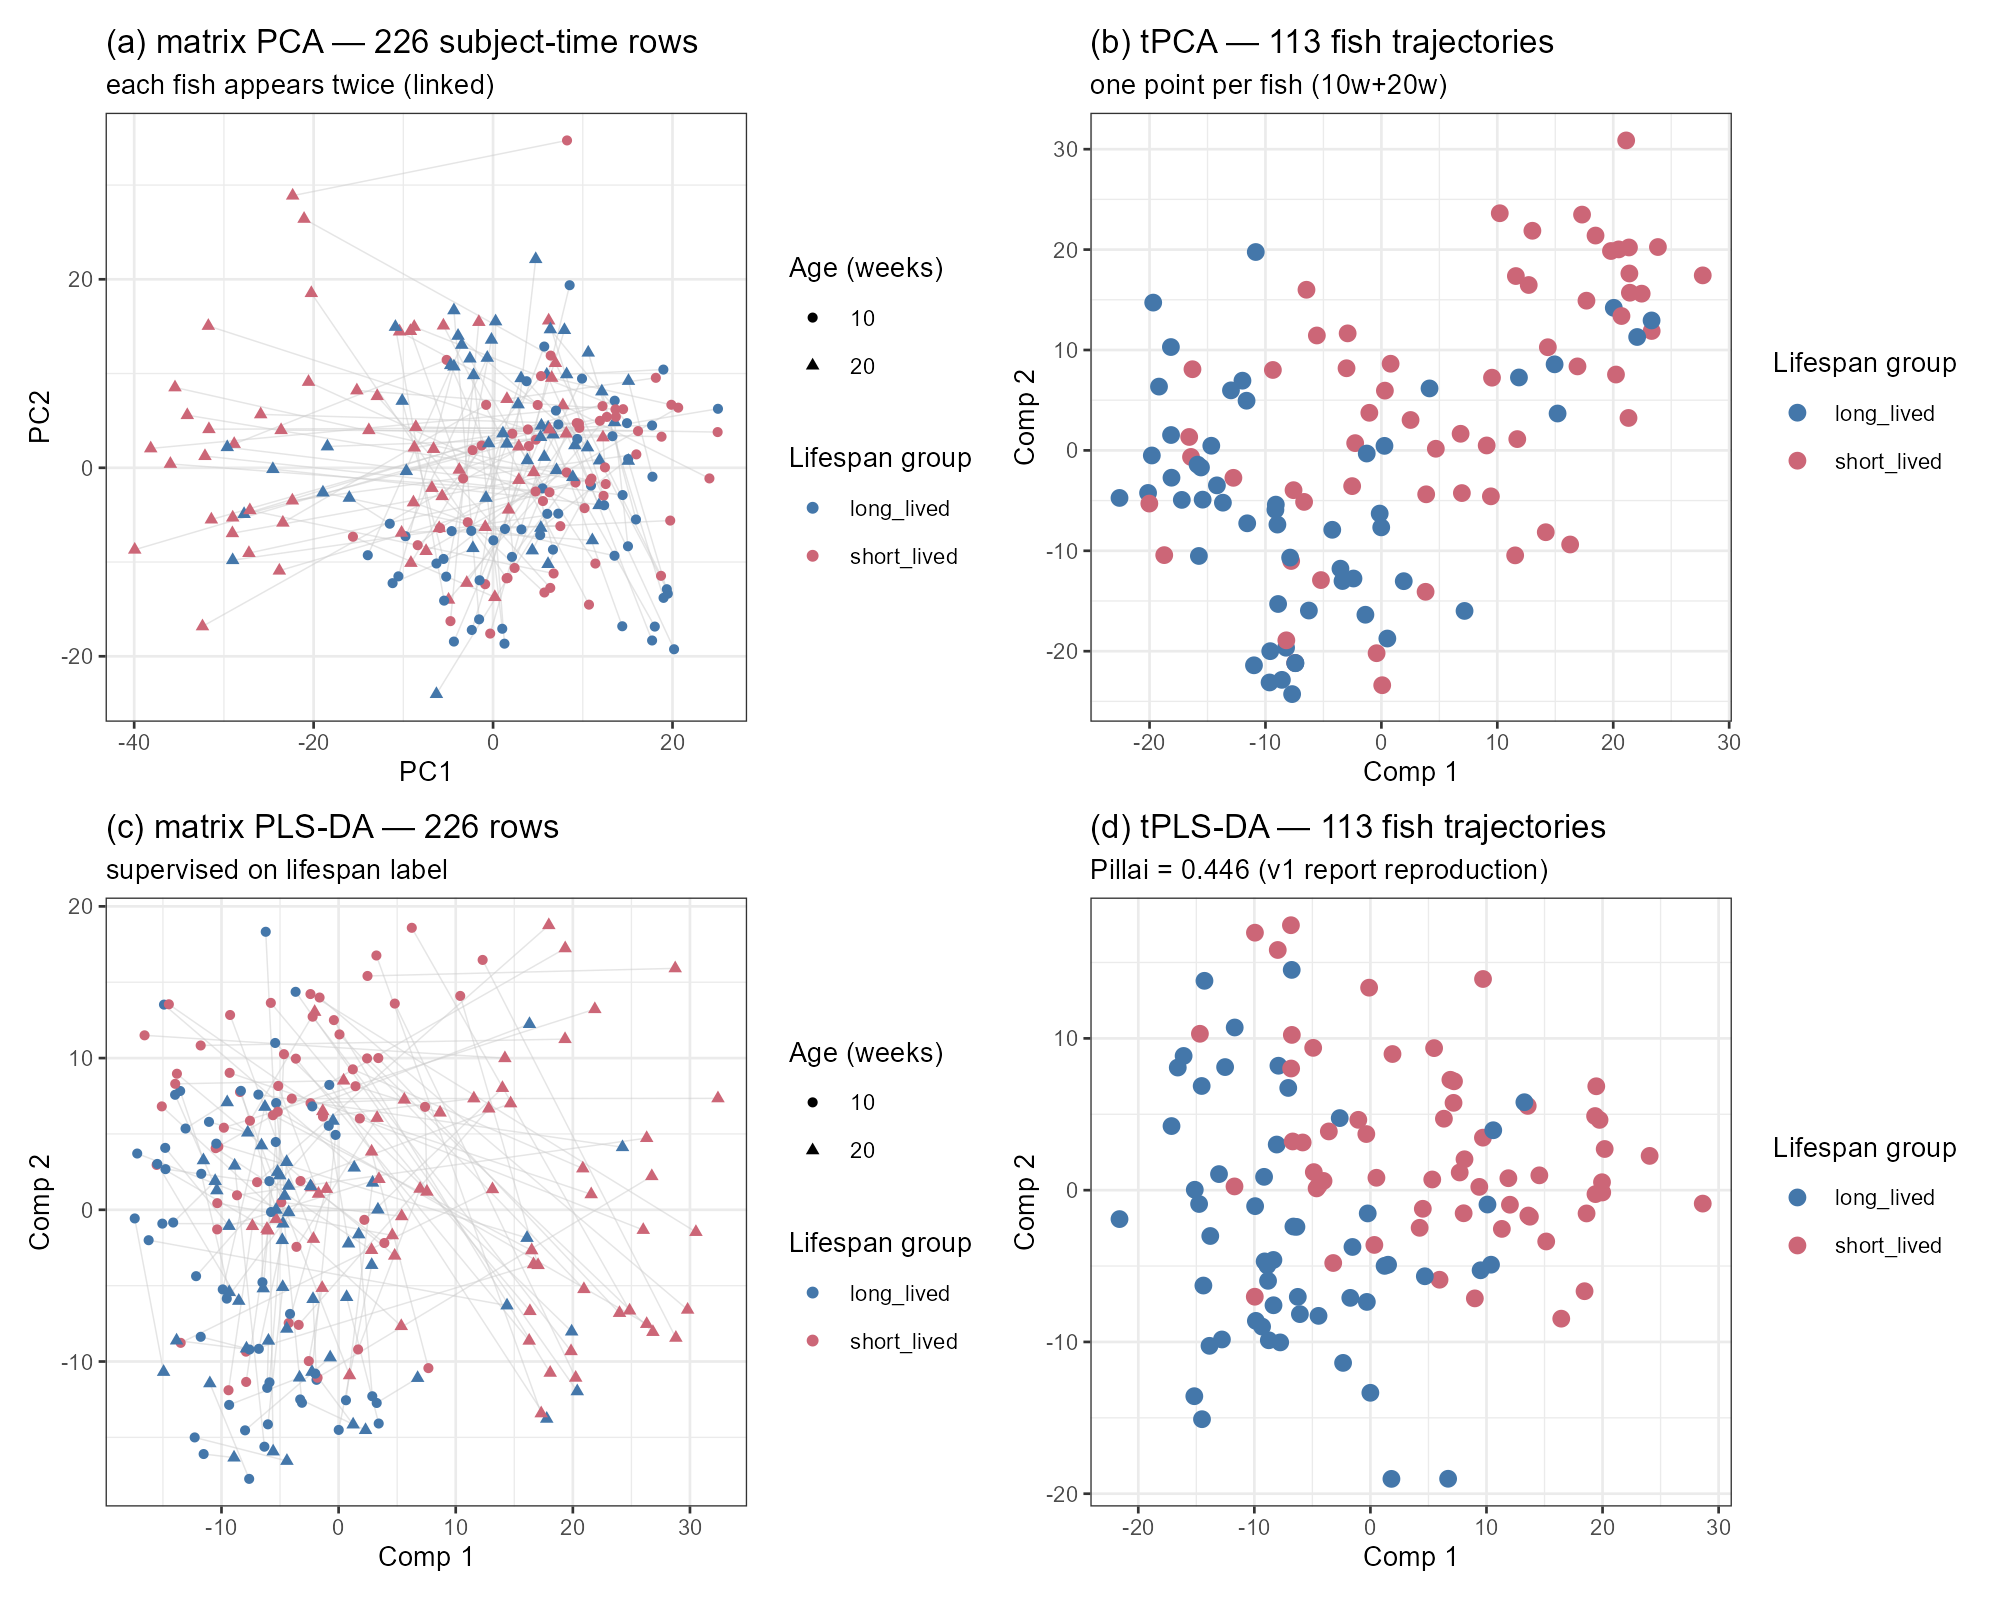
\includegraphics[keepaspectratio,alt={Matrix vs tensor views of the fish dataset. (a) matrix PCA and (c) matrix PLS-DA with one line per fish connecting its two time points; (b) tPCA and (d) tPLS-DA with one point per fish.}]{figures/FF1_fish_fragmentation.png}}
\caption{Matrix vs tensor views of the fish dataset. (a) matrix PCA and
(c) matrix PLS-DA with one line per fish connecting its two time points;
(b) tPCA and (d) tPLS-DA with one point per fish.}
\end{figure}

\begin{figure}
\centering
\pandocbounded{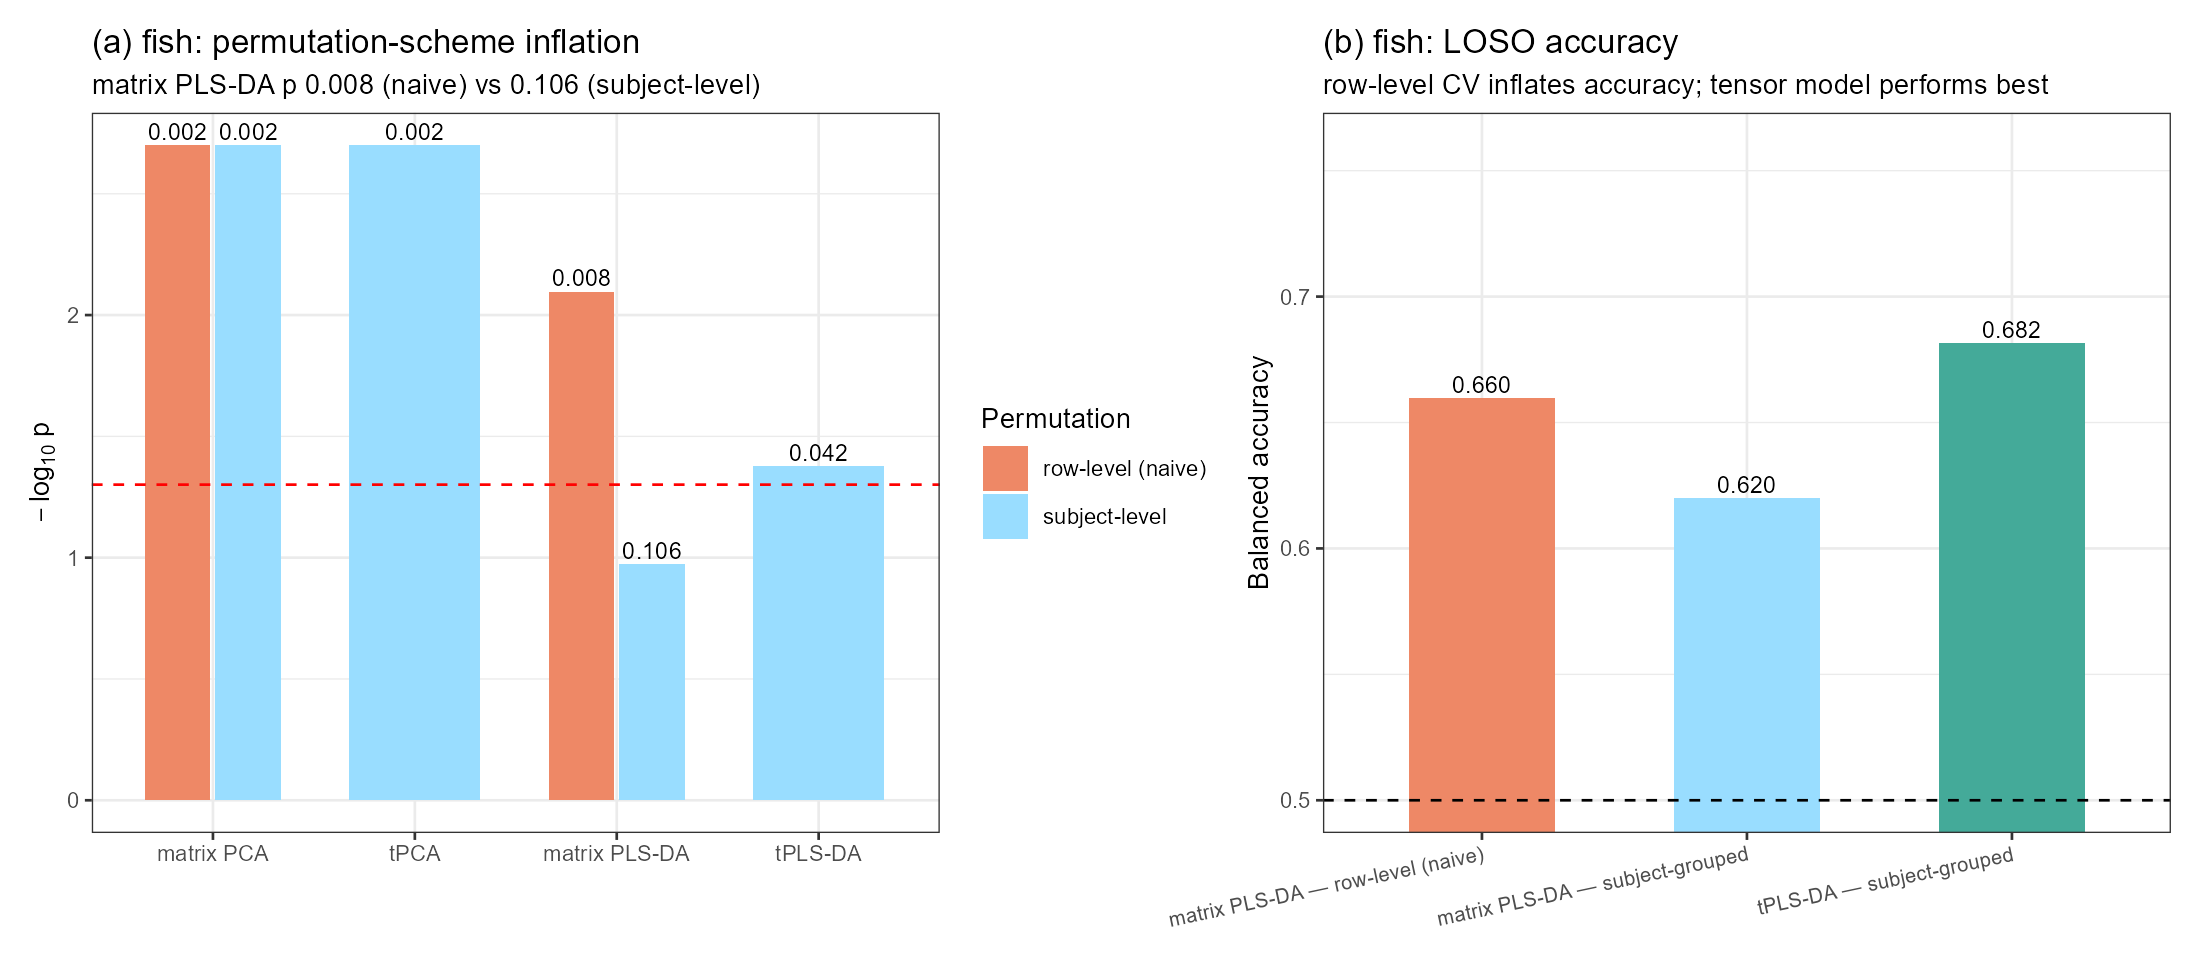
\includegraphics[keepaspectratio,alt={Fish inference diagnostics. (a) Pillai-trace permutation p-values (log scale) under row-level versus subject-level shuffling; (b) leave-one-subject-out balanced accuracy, row-level versus subject-grouped.}]{figures/FF2_fish_inflation_cv.png}}
\caption{Fish inference diagnostics. (a) Pillai-trace permutation
p-values (log scale) under row-level versus subject-level shuffling; (b)
leave-one-subject-out balanced accuracy, row-level versus
subject-grouped.}
\end{figure}

\subsection{4.2 Reassessing the lifespan
signal}\label{reassessing-the-lifespan-signal}

The earlier draft described the signal as ``connected to the
10-to-20-week trajectory''. Two structure-preserving checks correct that
statement (Figure FA2, Table 1):

\begin{itemize}
\tightlist
\item
  \textbf{Within-fish time reshuffle.} Swapping the two time points
  within each fish and refitting the whole pipeline does not reject the
  null (p = 0.150): the model performs nearly as well on temporally
  scrambled trajectories, so the data provide no evidence that the
  temporal ordering itself is required. This is an absence of evidence
  for a temporal-order effect rather than evidence that no dynamic
  component exists; with two time points and n = 113, a modest
  change-related contribution cannot be excluded. The audit model's
  subject-level label permutation, by contrast, gives p = 0.002 (\(R^2\)
  statistic; Table 1), indicating that the observed lifespan association
  is unlikely to arise under label shuffling. The tPLS-DA permutation of
  Section 4.1 tests a different statistic (Pillai under refitting) and
  is not directly comparable.
\item
  \textbf{Time-block ablation.} 10w only: \(R^2\) = 0.329; 20w only:
  0.488; 10w+20w: \textbf{0.541}; 10w+20w+delta: 0.505; delta only:
  0.412.
\end{itemize}

On the available evidence the signal is best described as
\textbf{level-based}: early-adulthood and 20-week expression levels
jointly carry the lifespan information, and the 10\$\to\$20-week change
adds no unique contribution (two time points still beat one: 0.541 vs
0.488). A modest change-related contribution cannot be excluded at this
sample size and with only two time points.

\begin{figure}
\centering
\pandocbounded{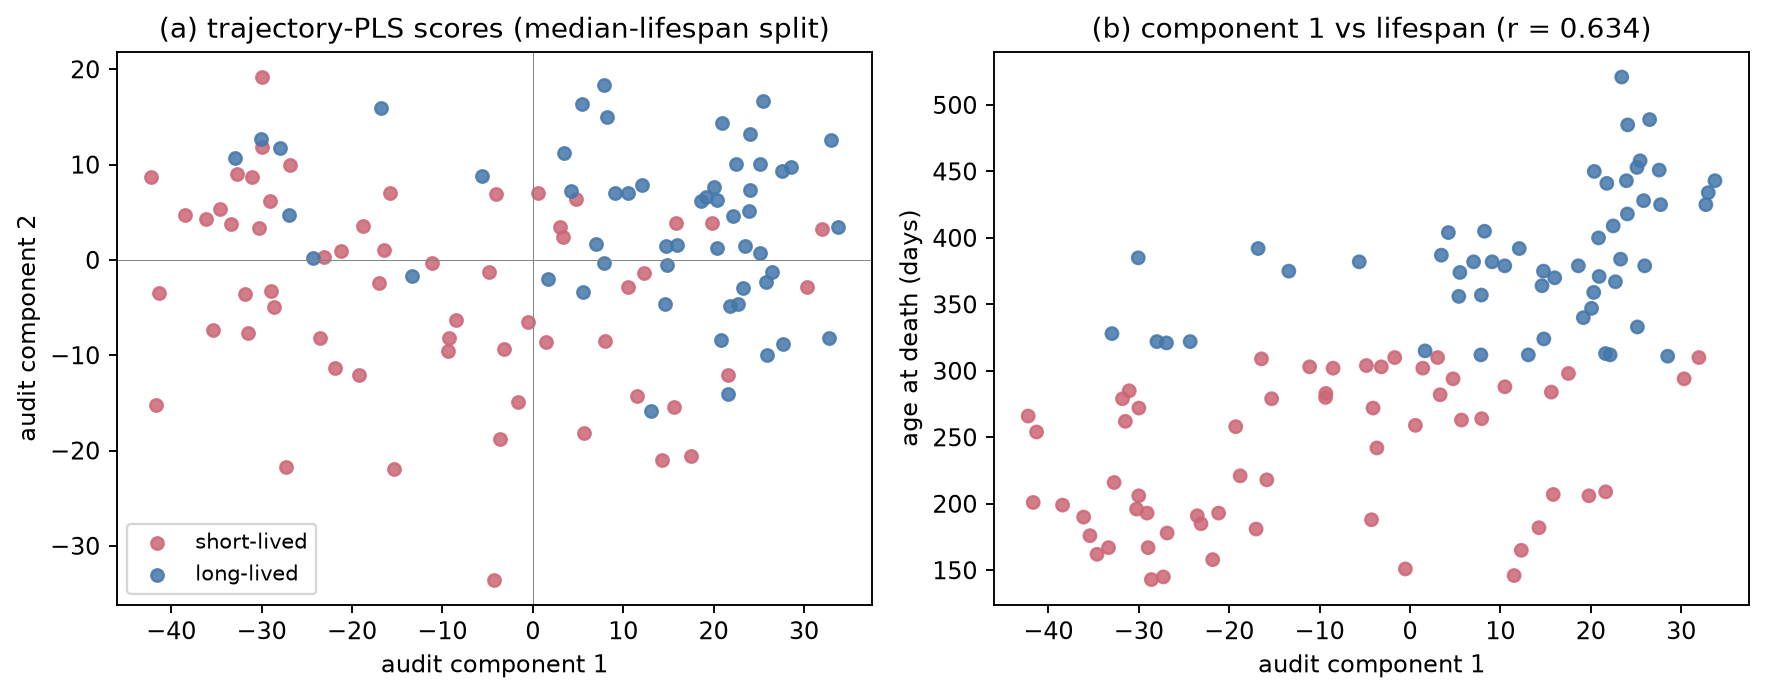
\includegraphics[keepaspectratio,alt={Independent audit of the fish lifespan signal: component scores against continuous age at death (audit model; r = 0.634 for component 1, with model-specific sign conventions --- see Section 4.1).}]{figures/FA1_fish_scores_age.png}}
\caption{Independent audit of the fish lifespan signal: component scores
against continuous age at death (audit model; r = 0.634 for component 1,
with model-specific sign conventions --- see Section 4.1).}
\end{figure}

\begin{figure}
\centering
\pandocbounded{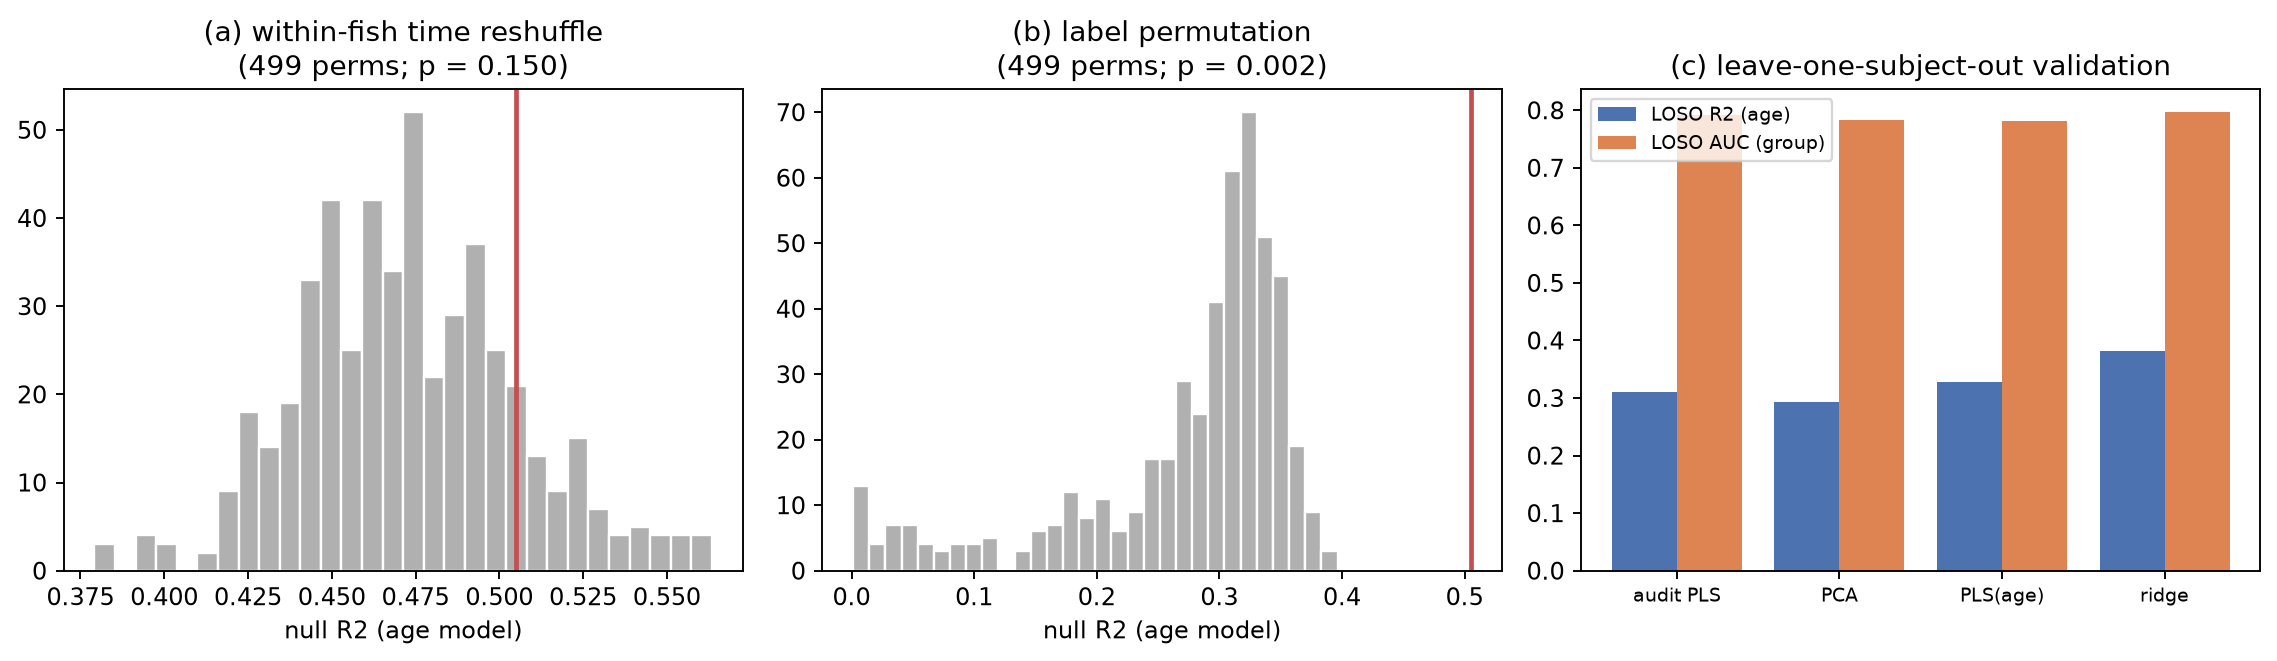
\includegraphics[keepaspectratio,alt={Structure-preserving permutation nulls and out-of-sample validation. (a) within-fish time reshuffle; (b) audit-model label permutation (R\^{}2 statistic); (c) leave-one-subject-out performance of the audit model and three baselines.}]{figures/FA2_fish_audit_nulls.png}}
\caption{Structure-preserving permutation nulls and out-of-sample
validation. (a) within-fish time reshuffle; (b) audit-model label
permutation (\(R^2\) statistic); (c) leave-one-subject-out performance
of the audit model and three baselines.}
\end{figure}

\textbf{Table 1. Fish main checks.}

{\def\LTcaptype{none} % do not increment counter
\begin{longtable}[]{@{}
  >{\raggedright\arraybackslash}p{(\linewidth - 6\tabcolsep) * \real{0.2500}}
  >{\raggedright\arraybackslash}p{(\linewidth - 6\tabcolsep) * \real{0.2500}}
  >{\raggedright\arraybackslash}p{(\linewidth - 6\tabcolsep) * \real{0.2500}}
  >{\raggedright\arraybackslash}p{(\linewidth - 6\tabcolsep) * \real{0.2500}}@{}}
\toprule\noalign{}
\begin{minipage}[b]{\linewidth}\raggedright
Analysis
\end{minipage} & \begin{minipage}[b]{\linewidth}\raggedright
Statistic
\end{minipage} & \begin{minipage}[b]{\linewidth}\raggedright
Value
\end{minipage} & \begin{minipage}[b]{\linewidth}\raggedright
p
\end{minipage} \\
\midrule\noalign{}
\endhead
\bottomrule\noalign{}
\endlastfoot
tPLS-DA group test (reproduction) & Pillai & 0.446 & 7.7
\(\times 10^{-15}\) \\
Label permutation, audit model (subject, 499) & \(R^2\) & 0.505 &
0.002 \\
Label permutation, tPLS-DA (refit under permutation, 499) & Pillai &
0.446 & 0.042 \\
Time reshuffle (within-fish, 499) & \(R^2\) & 0.505 & 0.150 \\
Continuous age, tPLS regression & \(R^2\) (in-sample) & 0.566 & 0.005
(perm) \\
Continuous age, tPLS regression (fold-safe) & LOSO CV \(R^2\) & -0.083 &
--- \\
Audit trajectory PLS, LOSO (fold-safe) & \(R^2\) / AUC & 0.308 / 0.792 &
--- \\
Ridge baseline (flattened 3,000 features), LOSO (fold-safe) & \(R^2\) /
AUC & 0.380 / 0.797 & --- \\
Bootstrap (fish) & \(R^2\) 95\% CI & {[}0.429, 0.661{]} & --- \\
\end{longtable}
}

The out-of-sample picture is consistent: in-sample \(R^2\) \(\approx\)
0.5--0.57 shrinks to \(\approx\) 0.31 under grouped LOSO for the
flattened audit model, and the two-component tensor regression does not
generalise at all (LOSO \(R^2\) = -0.083), even though held-out
component scores still correlate with age (r = -0.405). A simple ridge
regression on the flattened features matches or beats both. No
predictive claim is warranted; the dataset supports a replicated
association.

\subsection{4.3 Annotation closure: a circadian module and a diffused
complex I
theme}\label{annotation-closure-a-circadian-module-and-a-diffused-complex-i-theme}

The earlier report's largest interpretive gap --- anonymous killifish
gene identifiers --- was closed by mapping the full gene build. The four
bootstrap-stable genes are PAQR6, TUFT1A, COL10A1, and one identifier
that remains unannotated even in the primary source; they rank 3rd,
17th, 25th and 479th of 26,739 genes by delta-age association. More
importantly, the top loading genes include three core clock components
(\textbf{PER1, NPAS2, NR1D1}), and the clock kinase CSNK1E ranks 15th in
the top-50 delta-age FDR list; a targeted panel shows a coherent module:
\textbf{7 of the 8 canonical clock genes are FDR-significant with
consistent direction} (repressor arm NR1D1/CRY1/PER1/PER3 negative;
activator arm NPAS2/ARNTL/CLOCK positive; Figure FA4a). In plain terms,
the 10\$\to\$20-week expression change is more negative for
repressor-arm genes and more positive for activator-arm genes in
longer-lived fish. These are rank correlations between the change and
age at death: they describe a directional association of the change axis
with lifespan, not absolute up- or down-regulation of individual genes,
nor functional activation of the clock pathway. This change-oriented
panel analysis is distinct from the level-based lifespan model of
Section 4.2; the pattern connects to the aging--circadian literature and
is reported as hypothesis-generating.

The mitochondrial complex I hypothesis was tested directly. All 41
annotated complex I genes were located; \textbf{0/41 survive into the
1000 most variable genes} (they are too stable to be selected), 21/41
(51.2\%) show FDR-significant delta-age associations against a
transcriptome-wide background of 32.0\%, an enrichment of 1.60\(\times\)
(binomial p = 0.0083; median \textbar rho\textbar{} 0.235 vs 0.135,
Mann-Whitney p = 0.0015). Overall the theme is directionally consistent
but diffuse, and the original study's complex I claim is not recovered
from these data alone.

\begin{figure}
\centering
\pandocbounded{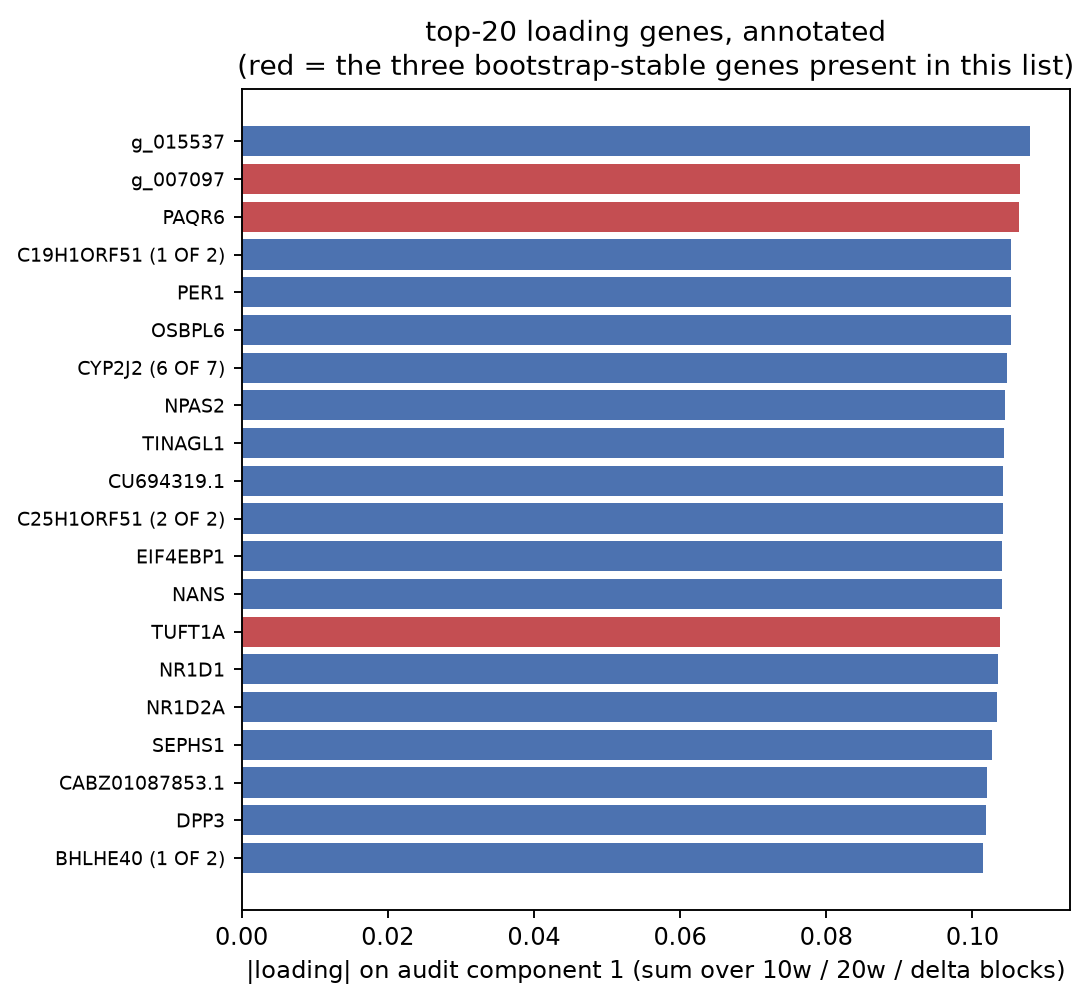
\includegraphics[keepaspectratio,alt={Annotated top-20 loading genes of the audit component 1; red marks the three bootstrap-stable genes present in this list (the fourth, COL10A1, lies outside the top 20).}]{figures/FA3_fish_annotated_loadings.png}}
\caption{Annotated top-20 loading genes of the audit component 1; red
marks the three bootstrap-stable genes present in this list (the fourth,
COL10A1, lies outside the top 20).}
\end{figure}

\begin{figure}
\centering
\pandocbounded{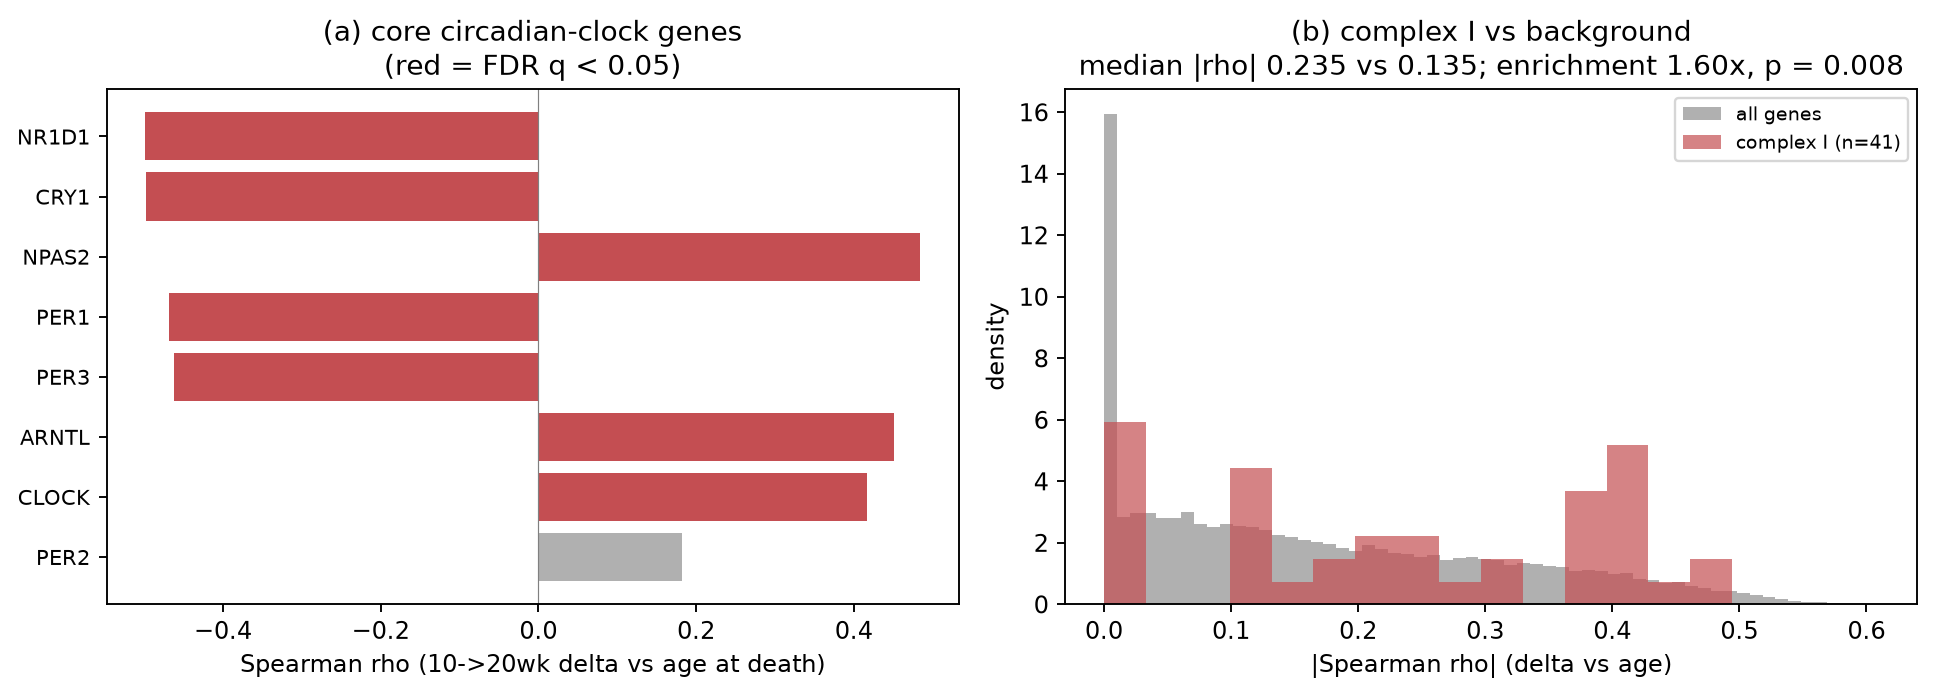
\includegraphics[keepaspectratio,alt={(a) core circadian-clock gene panel; (b) complex I genes against the transcriptome-wide background.}]{figures/FA4_fish_circadian_complexI.png}}
\caption{(a) core circadian-clock gene panel; (b) complex I genes
against the transcriptome-wide background.}
\end{figure}

\begin{figure}
\centering
\pandocbounded{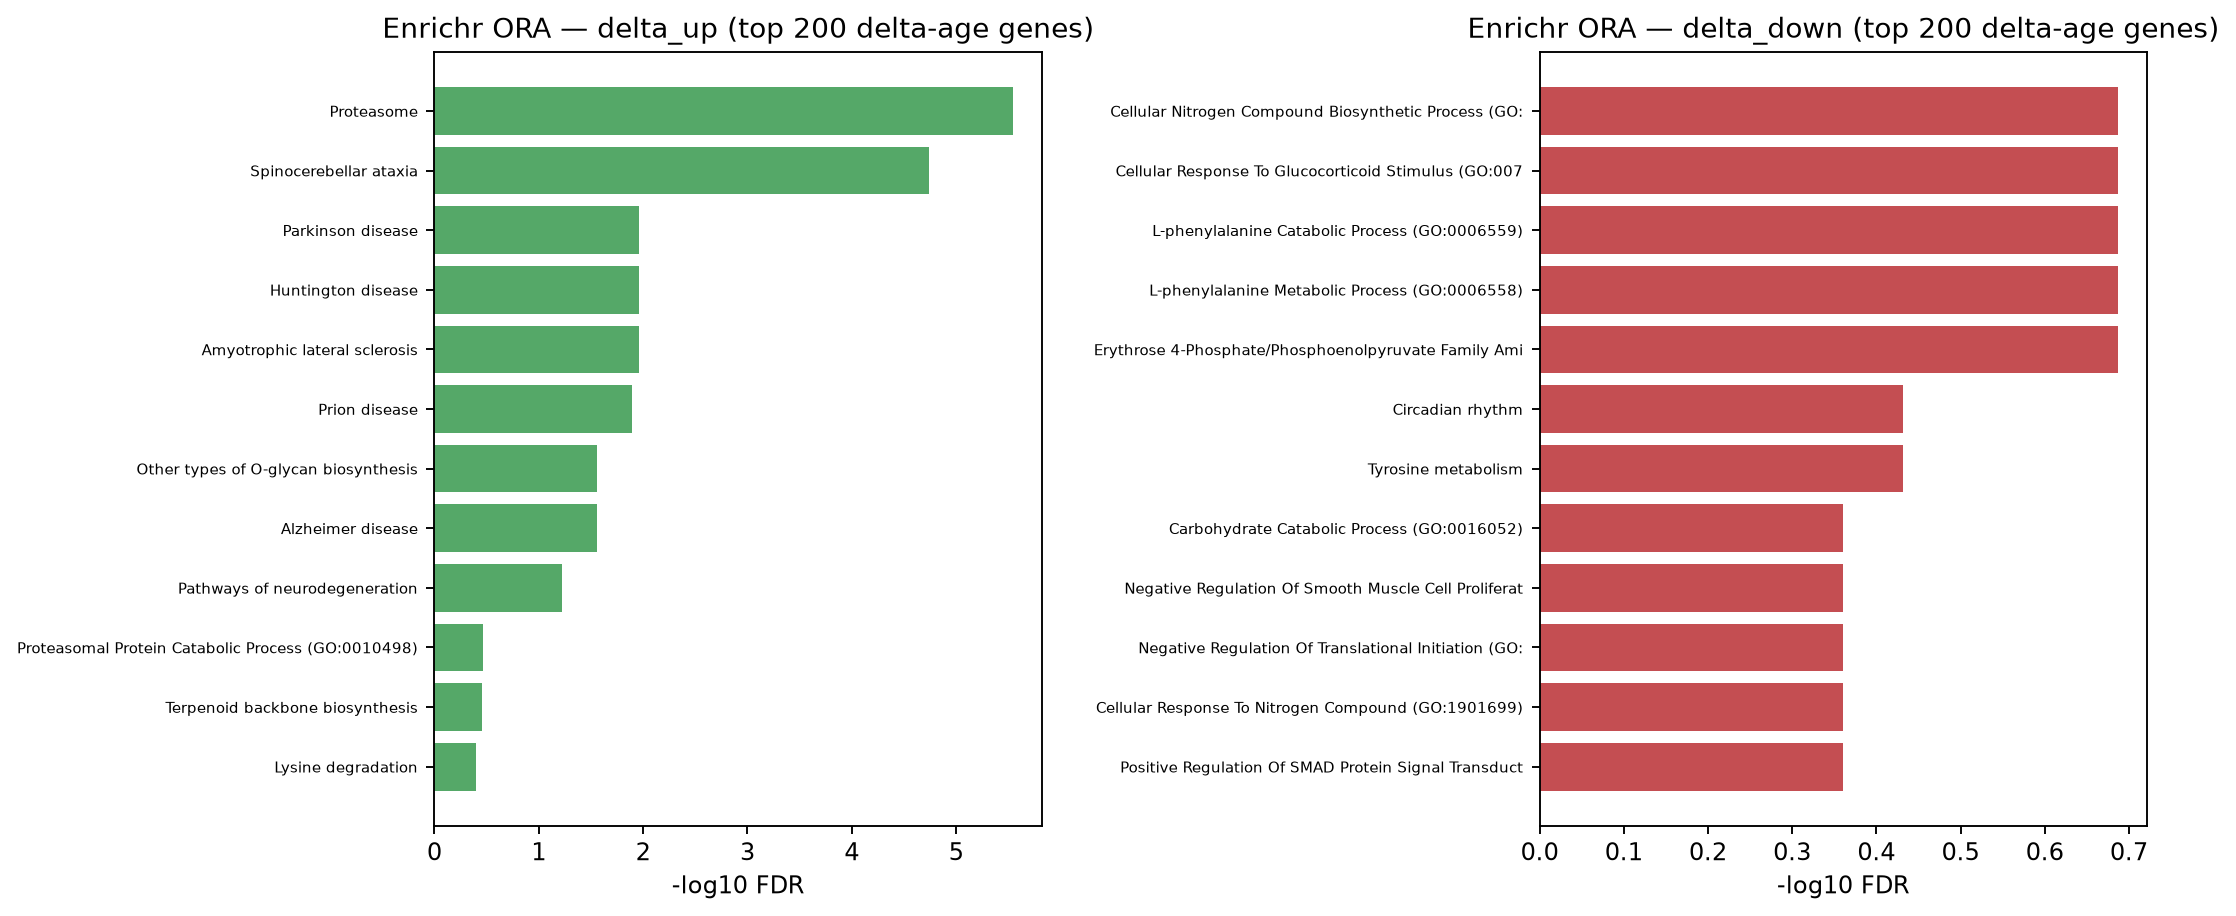
\includegraphics[keepaspectratio,alt={Enrichr over-representation analysis of the top 200 delta-age genes per direction against GO-BP 2023 and KEGG 2021; the delta-up direction is dominated by proteasome / ubiquitin-dependent degradation. No term passes FDR \textless{} 0.05 in the delta-down direction.}]{figures/FA5_fish_gsea.png}}
\caption{Enrichr over-representation analysis of the top 200 delta-age
genes per direction against GO-BP 2023 and KEGG 2021; the delta-up
direction is dominated by proteasome / ubiquitin-dependent degradation.
No term passes FDR \textless{} 0.05 in the delta-down direction.}
\end{figure}

Pathway enrichment on the same axis (Figure FA5) finds the
proteasome/ubiquitin axis up-regulated in longer-lived fish (KEGG
Proteasome, FDR = 3 \(\times 10^{-6}\)); the delta-down direction passes
no term. Gene-level FDR is diffuse (8,563/26,739 = 32.0\% of genes at q
\textless{} 0.05), so all conclusions are module-level statements, not
gene discoveries.

\subsection{4.4 Robustness and
sensitivity}\label{robustness-and-sensitivity}

The lifespan model is insensitive to the feature threshold (in-sample
\(R^2\) at 2 components: 0.512 / 0.505 / 0.495 at 500 / 1,000 / 2,000
genes) and improves smoothly with up to four components (up to 0.63),
with the caveat that more components mechanically raise in-sample fit.
Bootstrap resampling over fish gives \(R^2\) 95\% CI {[}0.429, 0.661{]}
and r(comp 1, age) CI {[}0.570, 0.753{]}.

\textbf{Interim conclusion (fish).} Early fin transcriptome
\emph{levels} carry a reproducible, cohort-validated association with
lifespan (in-sample \(R^2\) \(\approx\) 0.5, bootstrap CI excluding weak
effects), organised in coherent modules (circadian clock; proteasome)
rather than single genes; the 10\$\to\$20-week change adds nothing;
out-of-sample prediction is weak; and the complex I mechanism of the
original study is not recovered. The association is validated
\emph{within} this cohort only; external validation is required for any
predictive use.

\section{5 Results: vaccine transcriptome
(GSE79396)}\label{results-vaccine-transcriptome-gse79396}

\subsection{5.1 Exact reproduction and the value of the tensor
view}\label{exact-reproduction-and-the-value-of-the-tensor-view}

All earlier numbers were reproduced exactly (Section 3.2; component
scores correlate 1.0000). Figure FV1 shows the central representational
difference on this dataset (288 sample-time rows versus 72 subject
trajectories, days 0/1/3/7). Figure FV2 quantifies the inference
consequences: for the same matrix PLS-DA model, the naive row-level
permutation gives p = 0.002 while subject-level permutation gives p =
0.094, and row-level LOSO reports balanced accuracy 0.722 versus 0.644
with subject grouping. The subject-grouped tensor model reaches 0.685,
the best grouped accuracy in the comparison. Together these three
numbers show that flattening is not merely cosmetic: it changes p-values
by an order of magnitude and accuracy by \textasciitilde8 points. Both
grouped accuracies are robust to preprocessing provenance: re-deriving
feature selection and scaling inside every training fold leaves the
per-subject predictions unchanged.

\begin{figure}
\centering
\pandocbounded{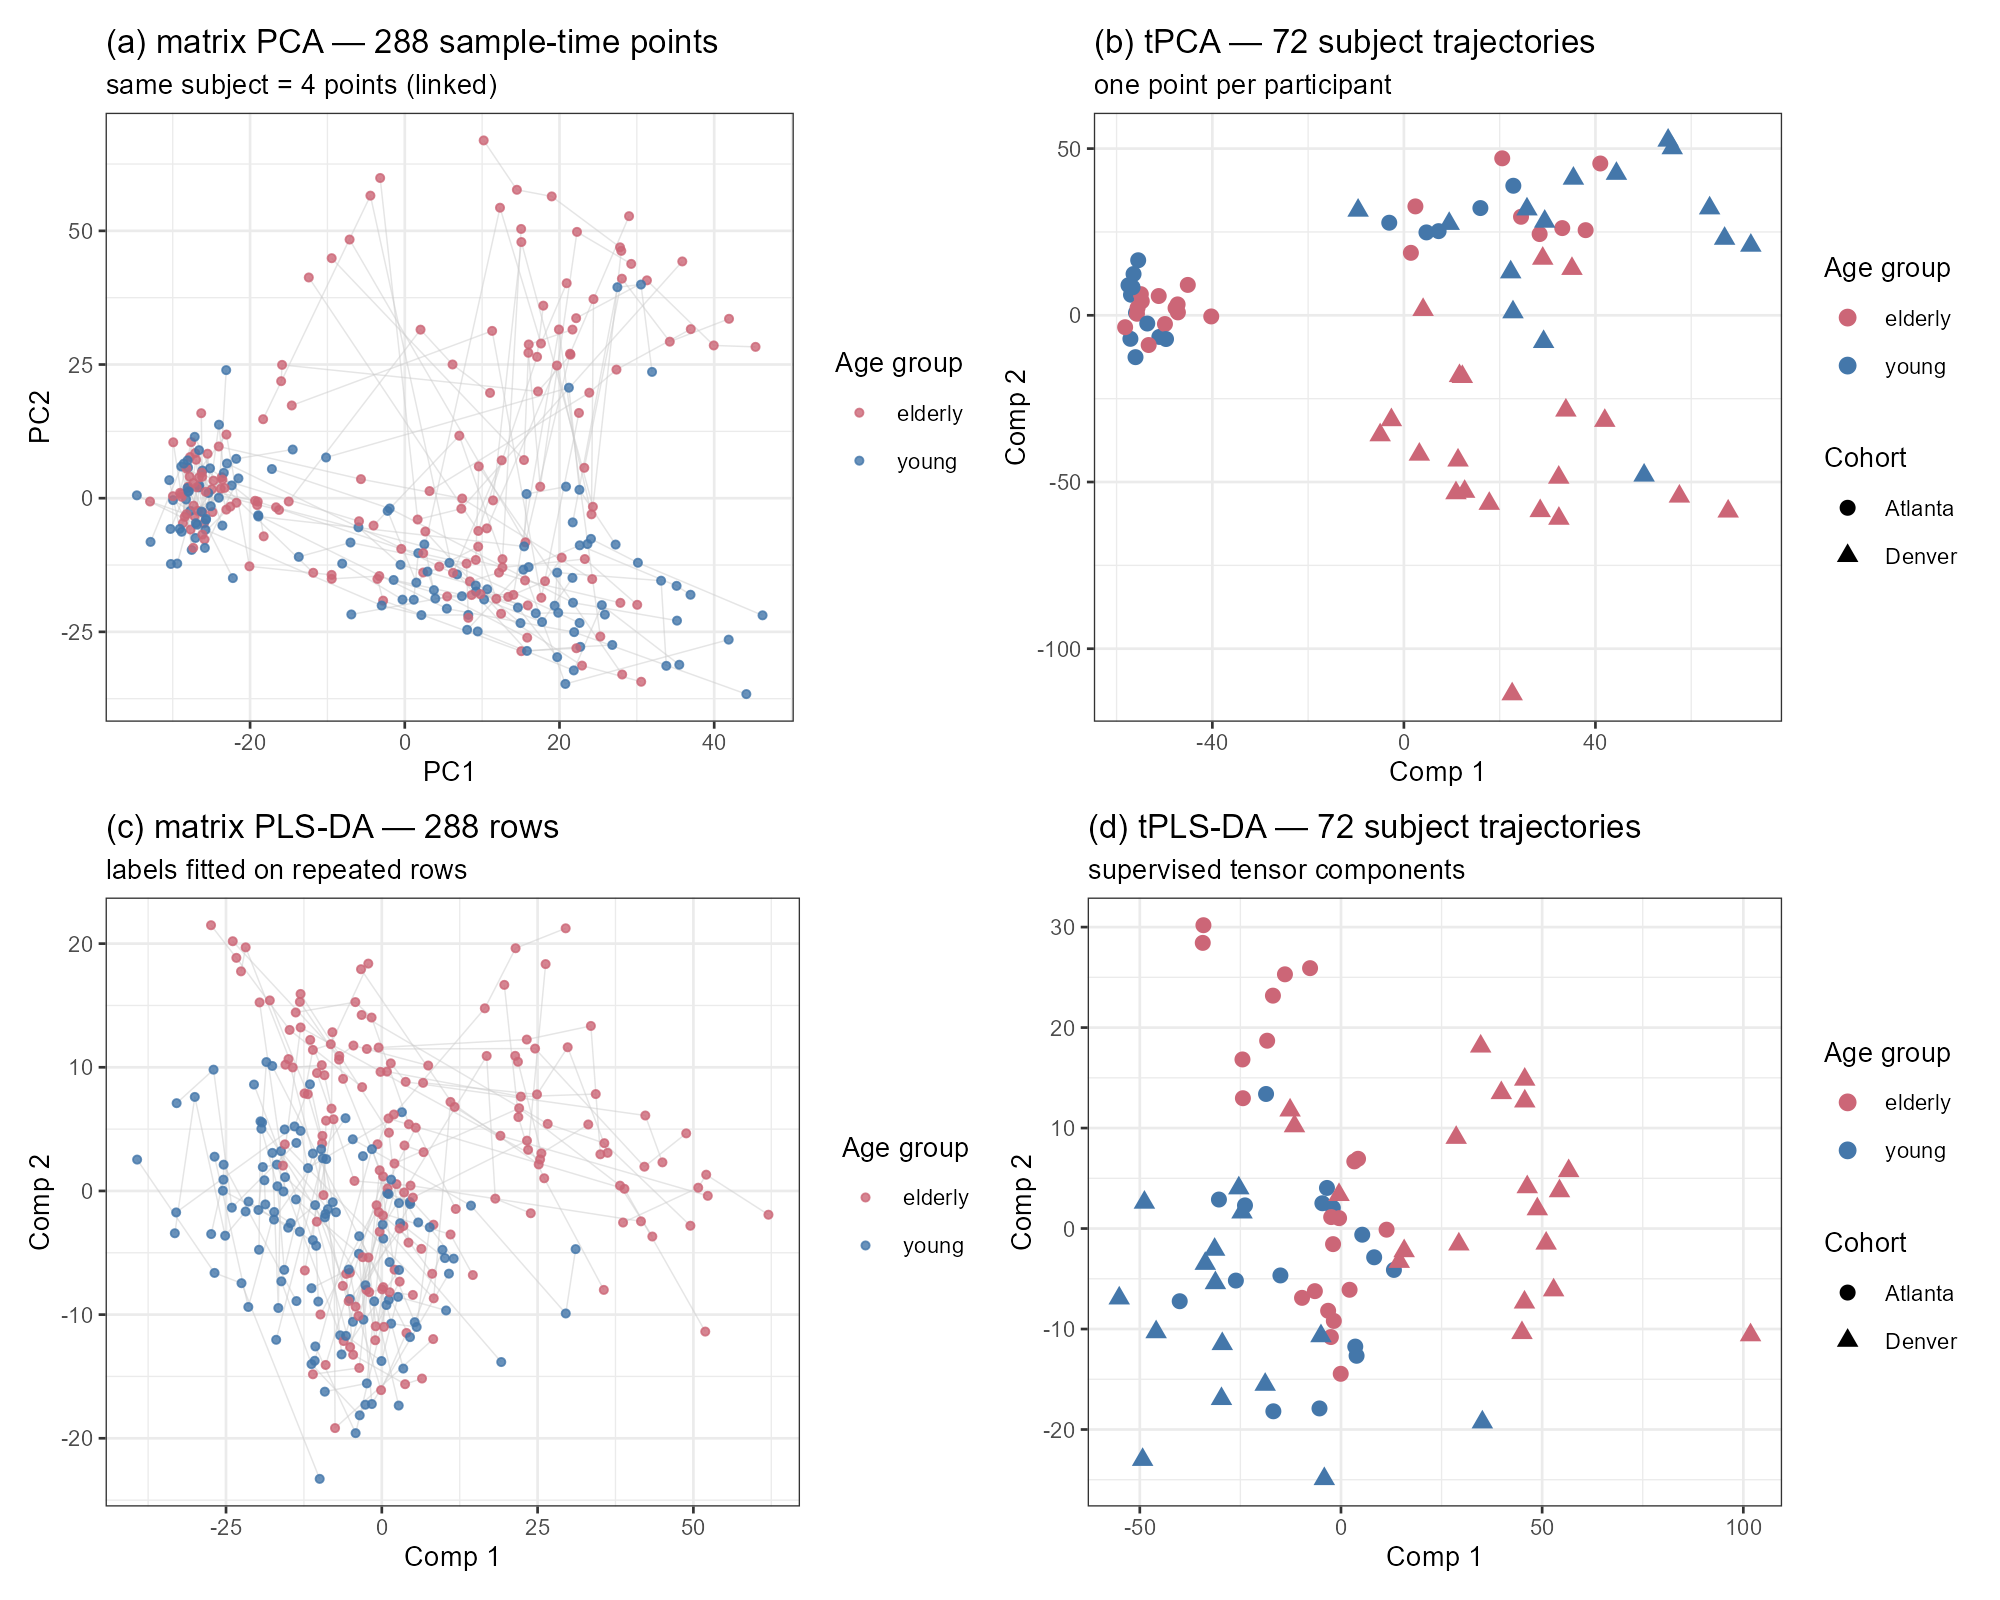
\includegraphics[keepaspectratio,alt={Subject-level representation. (a) matrix PCA and (c) matrix PLS-DA: 288 rows, each subject 4 points (linked); (b) tPCA and (d) tPLS-DA: 72 subject trajectories.}]{figures/FV1_fragmentation.png}}
\caption{Subject-level representation. (a) matrix PCA and (c) matrix
PLS-DA: 288 rows, each subject 4 points (linked); (b) tPCA and (d)
tPLS-DA: 72 subject trajectories.}
\end{figure}

\begin{figure}
\centering
\pandocbounded{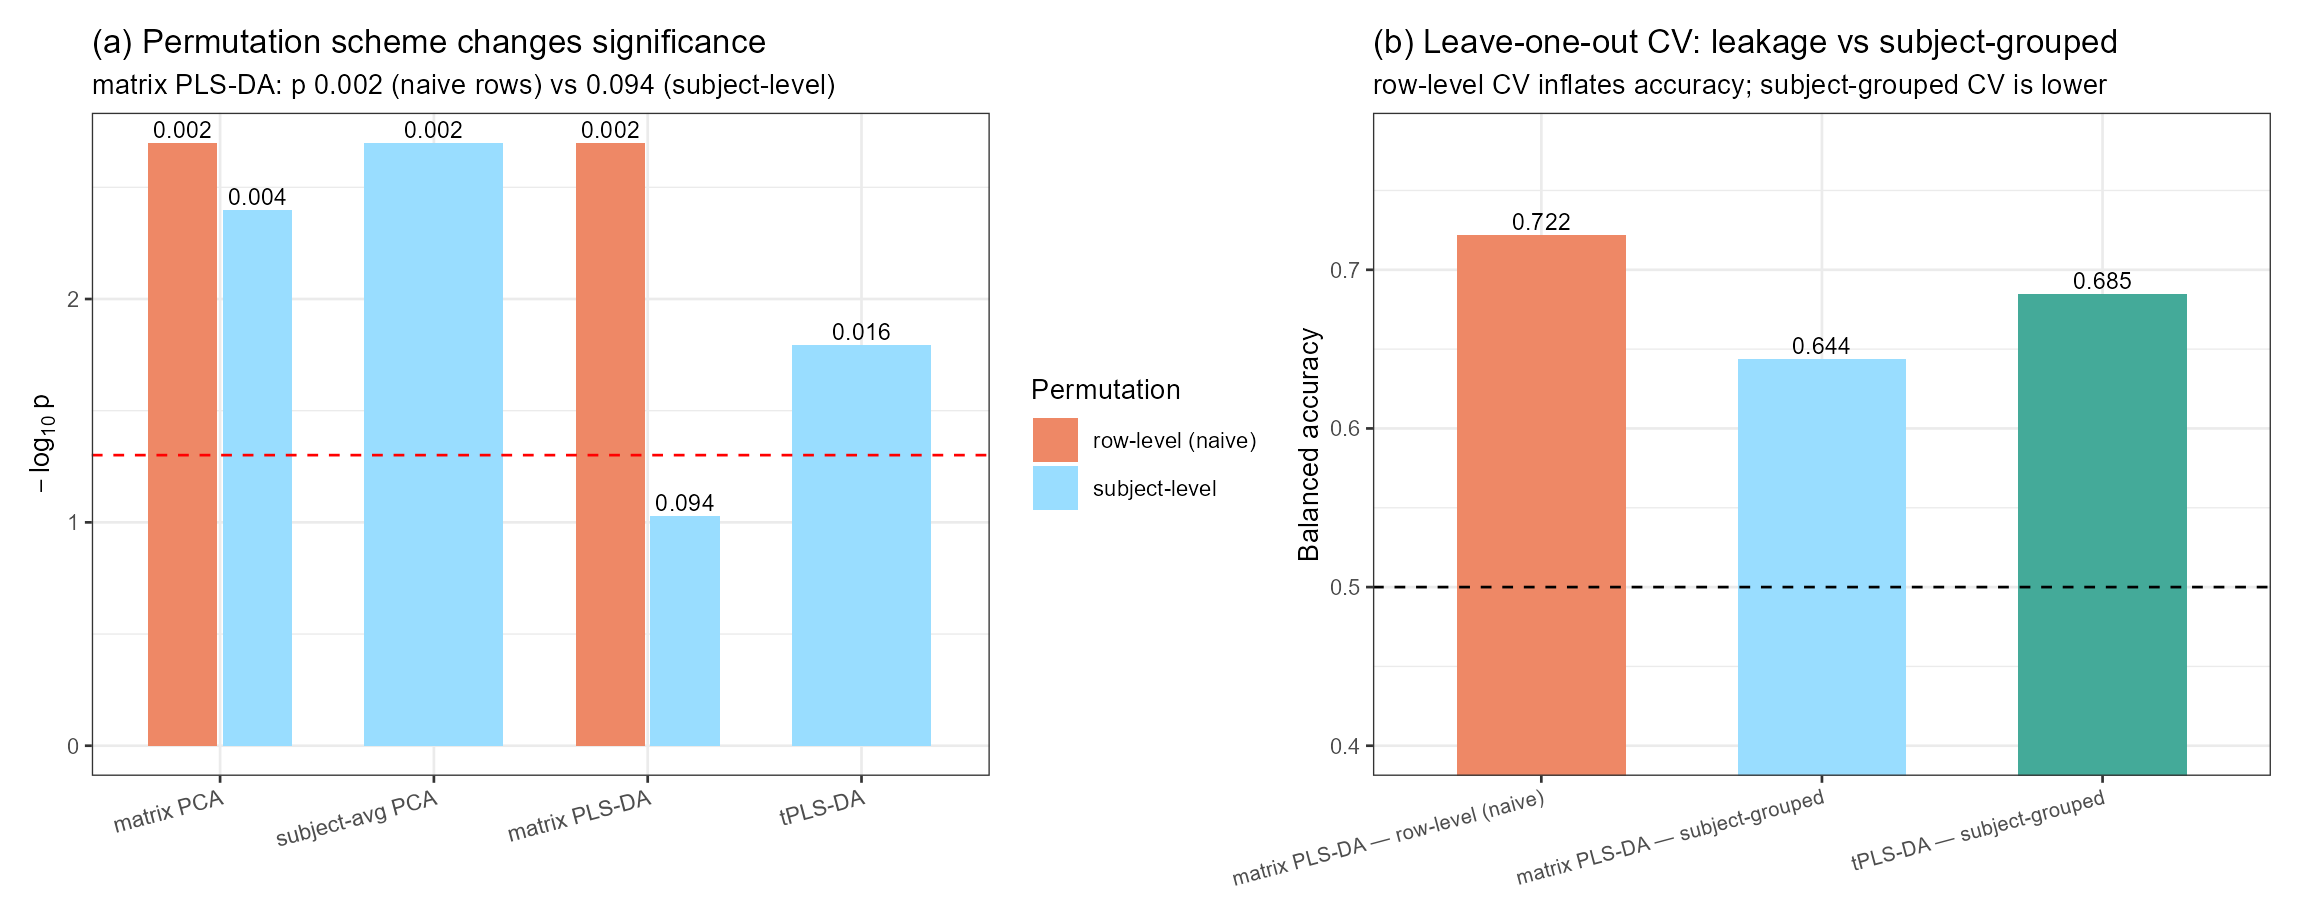
\includegraphics[keepaspectratio,alt={Inference diagnostics. (a) permutation-scheme inflation (matrix PLS-DA: 0.002 naive vs 0.094 subject-level); (b) leave-one-subject-out accuracy, row-level versus subject-grouped, and the tensor model.}]{figures/FV2_inflation_cv.png}}
\caption{Inference diagnostics. (a) permutation-scheme inflation (matrix
PLS-DA: 0.002 naive vs 0.094 subject-level); (b) leave-one-subject-out
accuracy, row-level versus subject-grouped, and the tensor model.}
\end{figure}

\subsection{5.2 The batch workflow: from cohort to processing
plate}\label{the-batch-workflow-from-cohort-to-processing-plate}

The tensorOmics paper's case study 3 established the workflow ``tPCA
detects batch structure, PLSDA-batch corrects, biology re-emerges''.
Applied here, the audit pushed one level deeper than the available batch
label (Figure FV3):

\begin{itemize}
\tightlist
\item
  \textbf{Cohort.} tPCA separates Atlanta from Denver (Pillai = 0.624, p
  = 2.3 \(\times 10^{-15}\); \(\eta^2\) = 0.49 on component 1).
  Cohort-level ComBat removes this structure (Pillai = 0.002, p = 0.93)
  and the unsupervised age association survives (permutation p = 0.003).
  Applying PLSDA-batch to the ComBat output --- a layered correction
  rather than an independent replication --- leaves the residual cohort
  structure equally low (\(\eta^2\) \(\approx\) 0.0002). At this point
  the analysis resembles the original report's conclusion.
\item
  \textbf{Plate.} Extracting the processing-plate serials from the CEL
  file names revealed three plates nested within cohorts and strongly
  confounded with age (plate 8000000153: 11 young/13 elderly;
  8000001652: 16/8; 8000013046: 4/20). The plate structure is the
  strongest technical factor in the tensor (tPCA Pillai = 1.45, p
  \(\approx\) 1 \(\times 10^{-37}\), stronger than cohort), and because
  each subject's four visits sit on the same plate, it is invisible to
  cohort-level correction.
\item
  \textbf{After plate-level correction} (ComBat with plate as batch,
  age/sex preserved): the age association of the transcriptome collapses
  --- tPCA permutation p = 0.177 (from 0.003), five-component tPCA p =
  0.57 (Pillai = 0.056), supervised tPLS-DA permutation p = 0.327. The
  non-destructive complement (age + plate + sex covariate adjustment of
  the original components) agrees for the unsupervised space (age MANOVA
  p = 0.295). Within the one plate that mixes cohorts and age groups (n
  = 24), the age test is also null (p = 0.158).
\end{itemize}

\begin{figure}
\centering
\pandocbounded{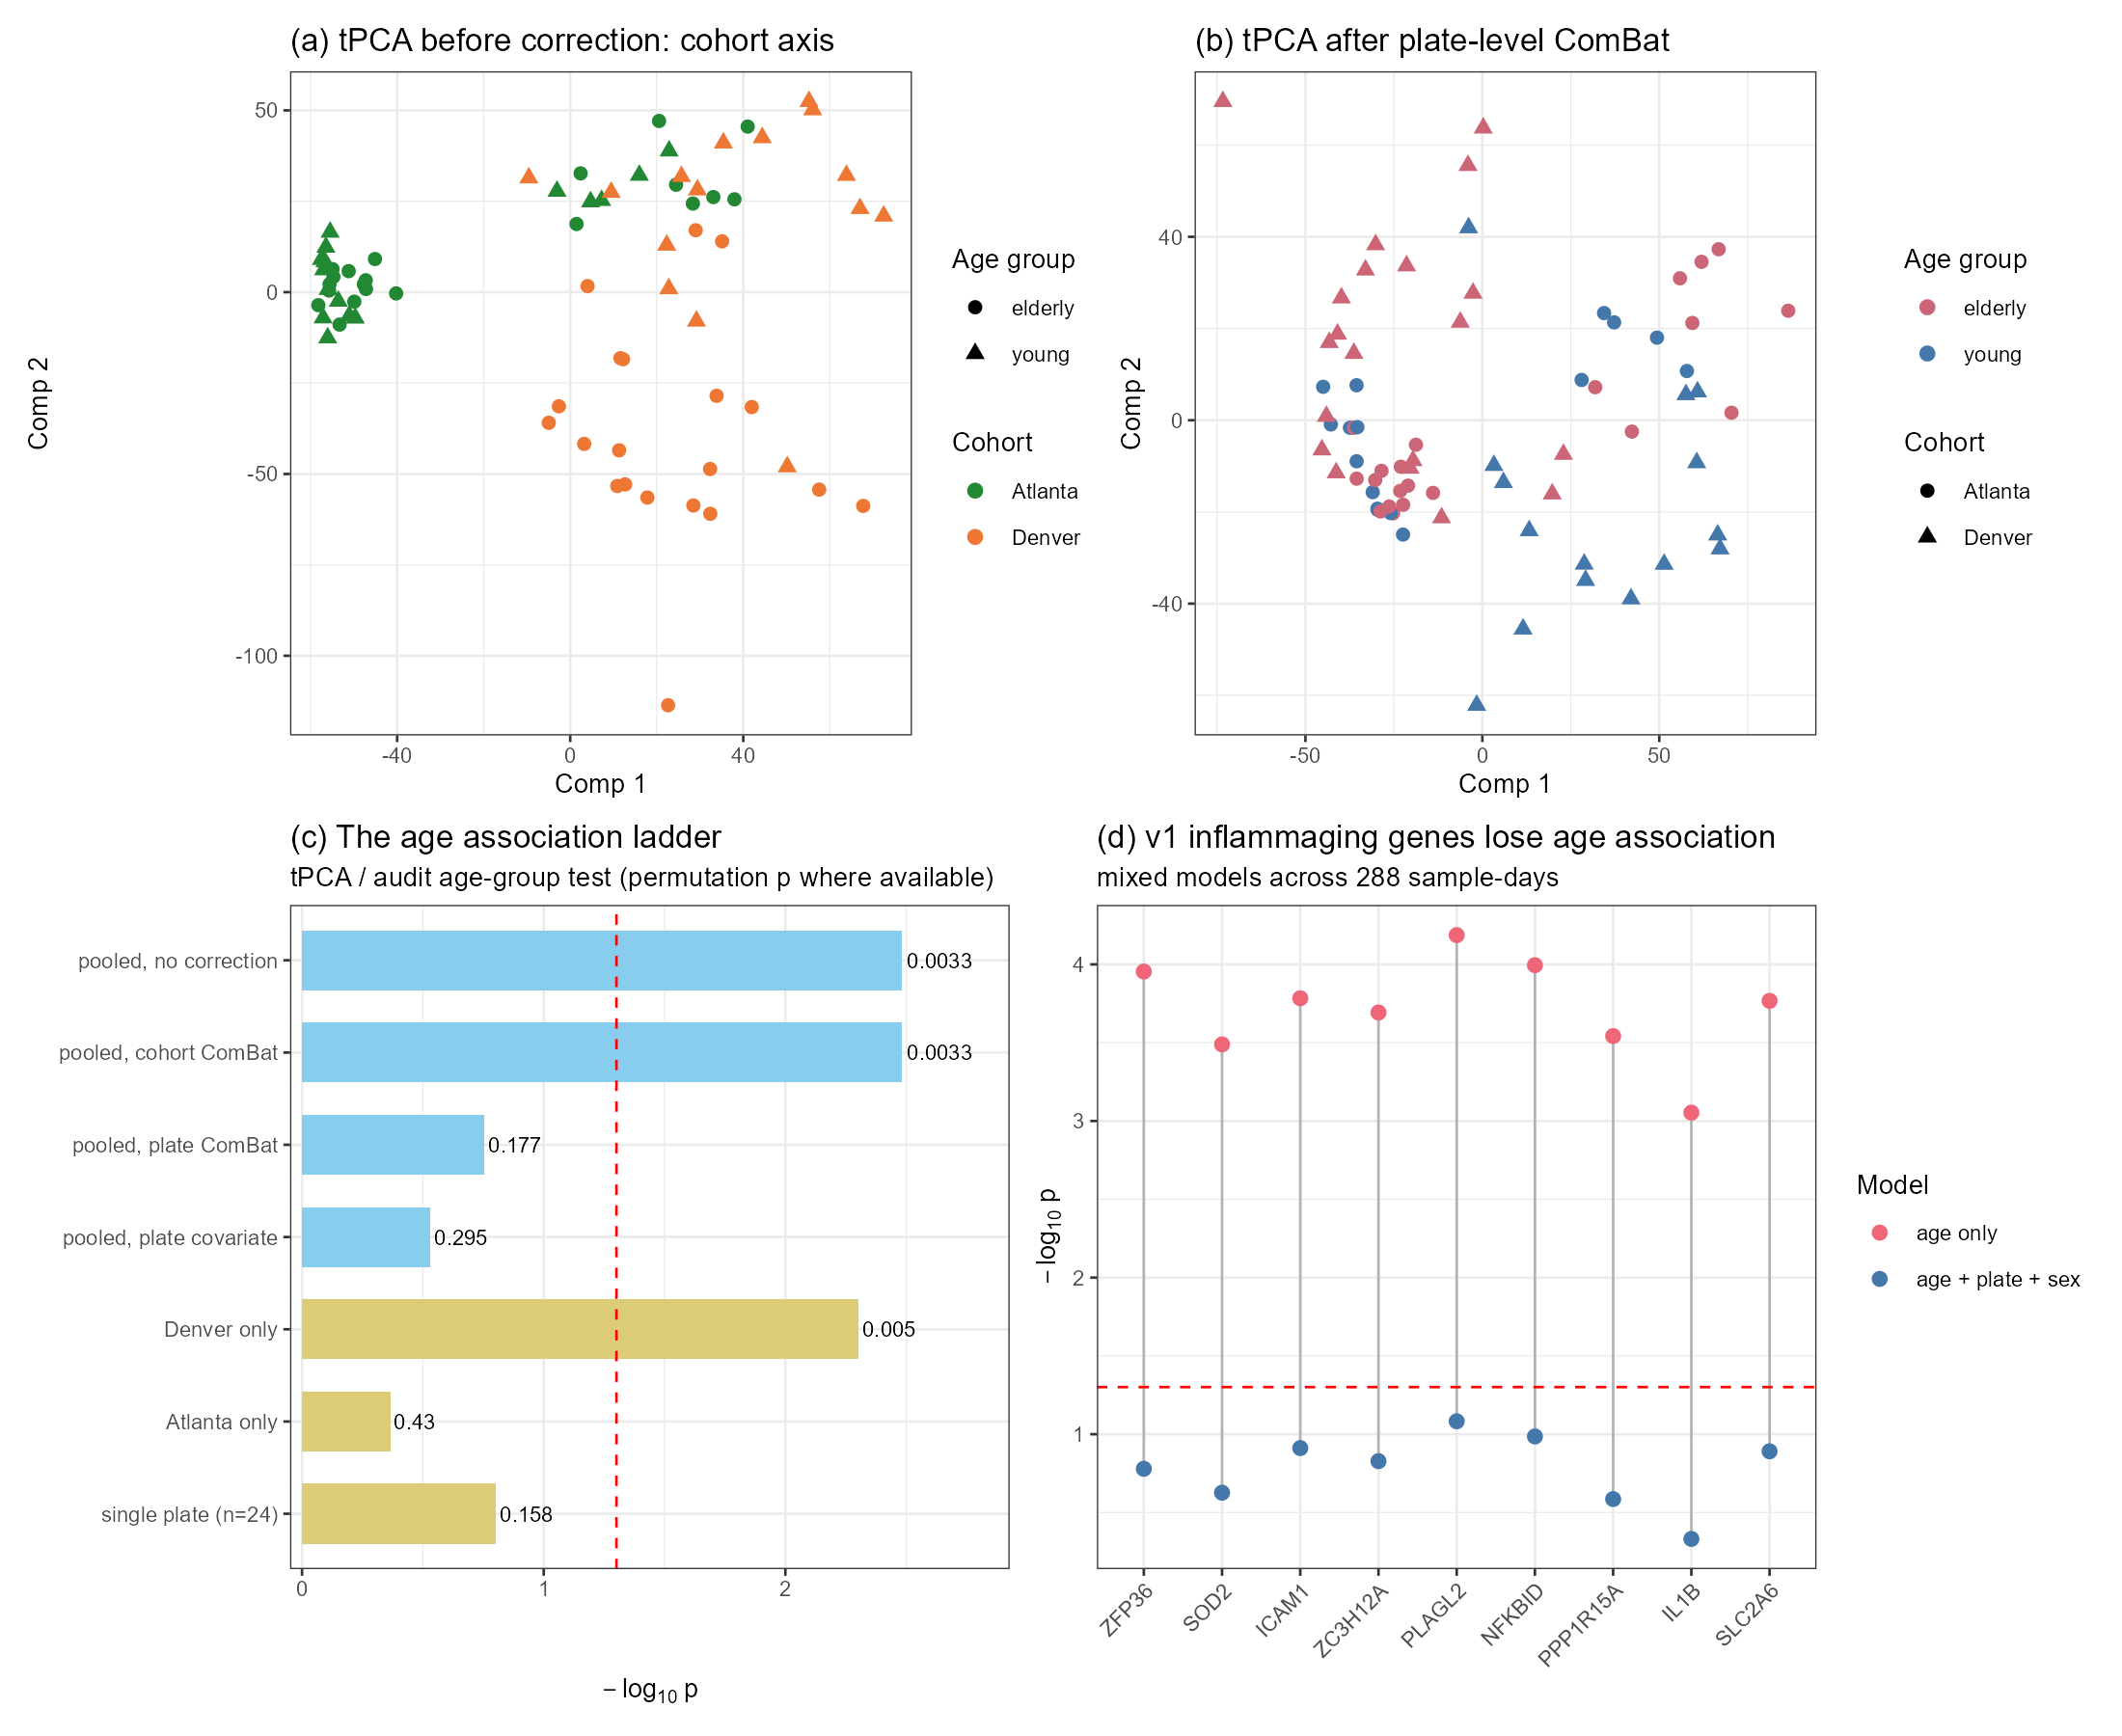
\includegraphics[keepaspectratio,alt={Batch audit. (a) tPCA before correction: the cohort axis; (b) tPCA after plate-level ComBat; (c) the age-association ladder across correction levels and within-batch replications; (d) the original inflammaging panel before vs after plate adjustment.}]{figures/FV3_batch_ladder.png}}
\caption{Batch audit. (a) tPCA before correction: the cohort axis; (b)
tPCA after plate-level ComBat; (c) the age-association ladder across
correction levels and within-batch replications; (d) the original
inflammaging panel before vs after plate adjustment.}
\end{figure}

\subsection{5.3 The age axis and its gene content do not
survive}\label{the-age-axis-and-its-gene-content-do-not-survive}

The earlier version of this report interpreted component 2 as an
age-associated inflammaging axis, enriched for inflammatory,
oxidative-stress and lipid/sterol terms. Exposed to the plate audit,
that interpretation does not hold (Figure FV3d):

\begin{itemize}
\tightlist
\item
  All nine highlight genes (ZFP36, SOD2, ICAM1, ZC3H12A, PLAGL2, NFKBID,
  PPP1R15A, IL1B, SLC2A6) lose significance in mixed models with plate
  and sex (age-only p = 6.5 \(\times 10^{-5}\)--8.8 \(\times 10^{-4}\);
  adjusted p = 0.083--0.466); effect sizes shrink 3--7\(\times\) (e.g.,
  ICAM1: \(\beta\) 0.91 \(\to\) 0.28).
\item
  No blood transcription module shows an age effect after plate
  adjustment (best raw p = 0.0055; FDR = 0.99 across 1,038 module--time
  combinations).
\item
  The axis is also site-heterogeneous: within Denver the age association
  is strong (Pillai = 0.606, permutation p = 0.005; fold-safe LOSO
  balanced accuracy 0.78--0.79), within Atlanta it is absent (Pillai =
  0.044, p = 0.43; fold-safe LOSO 0.41--0.52; 5-component check p =
  0.91). The Denver signal follows its plate composition (20/24 elderly
  on one plate), so the between-site contrast is itself consistent with
  the plate explanation.
\item
  A day-resolved axis score built from the supervised top-20 features
  shows a persistent age offset with no temporal dynamics (age p = 0.006
  with plate/sex in the model; age \(\times\) day interaction p = 0.68;
  53\% of the score's variance lies between subjects). Because the
  feature set was selected on the same data, this is descriptive rather
  than confirmatory.
\end{itemize}

\textbf{Conclusion for this dataset:} the apparent transcriptomic age
axis of GSE79396 is not separable from processing-plate batch structure
at n = 72. The pooled age signal, the inflammaging gene panel and the
module-level associations must be treated as confounded; the defensible
statements are negative and methodological.

\subsection{5.4 Boundary analysis: response prediction and
power}\label{boundary-analysis-response-prediction-and-power}

The earlier draft reported that response-level models (IgG day 30/0;
CXCR3+ Tfh day 7/0) fitted in-sample but failed out of sample. The
present analysis quantifies this boundary rather than only recording
failure: with n = 72 the minimum detectable \textbar r\textbar{} at 80\%
power is 0.325; the observed correlations of the age axis with IgG day
30/0 are r = -0.126 (95\% CI {[}-0.245, 0.244{]}) and with Tfh r = 0.081
(n = 34, CI {[}-0.343, 0.325{]}). The confidence intervals are wide and
include moderate effects, so the correct statement is ``this design
cannot exclude a moderate response association'' rather than ``no
association exists''. Combined with the batch findings, no
response-prediction claim is supportable.

\section{6 Results: multi-block integration
(transcriptome--metabolome)}\label{results-multi-block-integration-transcriptomemetabolome}

To exercise the framework's multi-omic capabilities, the vaccine
transcriptome was integrated with the study's own subject-level
metabolomics, restricted to the matching days 0/1/3/7 and 72 subjects
(top 500 transcriptome features; top 250 positive-mode and 250
negative-mode metabolites by variance; features z-scored). Figure FV4
summarises the results.

\begin{itemize}
\tightlist
\item
  \textbf{Unsupervised integration (tPLS canonical).} A strong shared
  axis links the two blocks: the subject scores of component 1 correlate
  at r = 0.833 (pairing permutation p = 0.01), component 2 at r = 0.658.
\item
  \textbf{Supervised integration (block.tPLS-DA, three blocks).} The
  transcriptome block separates age groups (Pillai = 0.165, p = 0.002;
  permutation p = 0.010); the metabolite blocks are weaker (p = 0.16 and
  0.053).
\item
  \textbf{The batch lens applies to integration too.} Alignment analysis
  shows the shared axis tracks plate structure (transcriptome-side plate
  Pillai = 1.53, p \(\approx\) 3 \(\times 10^{-42}\); metabolome-side
  plate Pillai = 1.18) and cohort (0.61 / 0.75) far more than age (0.165
  / 0.076). With the transcriptome plate-corrected, the shared-axis
  correlation falls from 0.833 to 0.444 and the corrected axis aligns
  with none of the labels (age p = 0.88, cohort p = 0.09, plate p =
  0.93). The metabolite block itself shows the same hierarchy (cohort p
  = 2.8 \(\times 10^{-15}\); plate p = 4.3 \(\times 10^{-12}\); age p =
  0.169).
\item
  The cross-layer correlation structure (top 30 \(\times\) 30 feature
  pairs per time point; Figure FV4c) is available as data for the
  report; its strongest components reflect the coordinated
  technical/cohort structure rather than age biology.
\end{itemize}

\begin{figure}
\centering
\pandocbounded{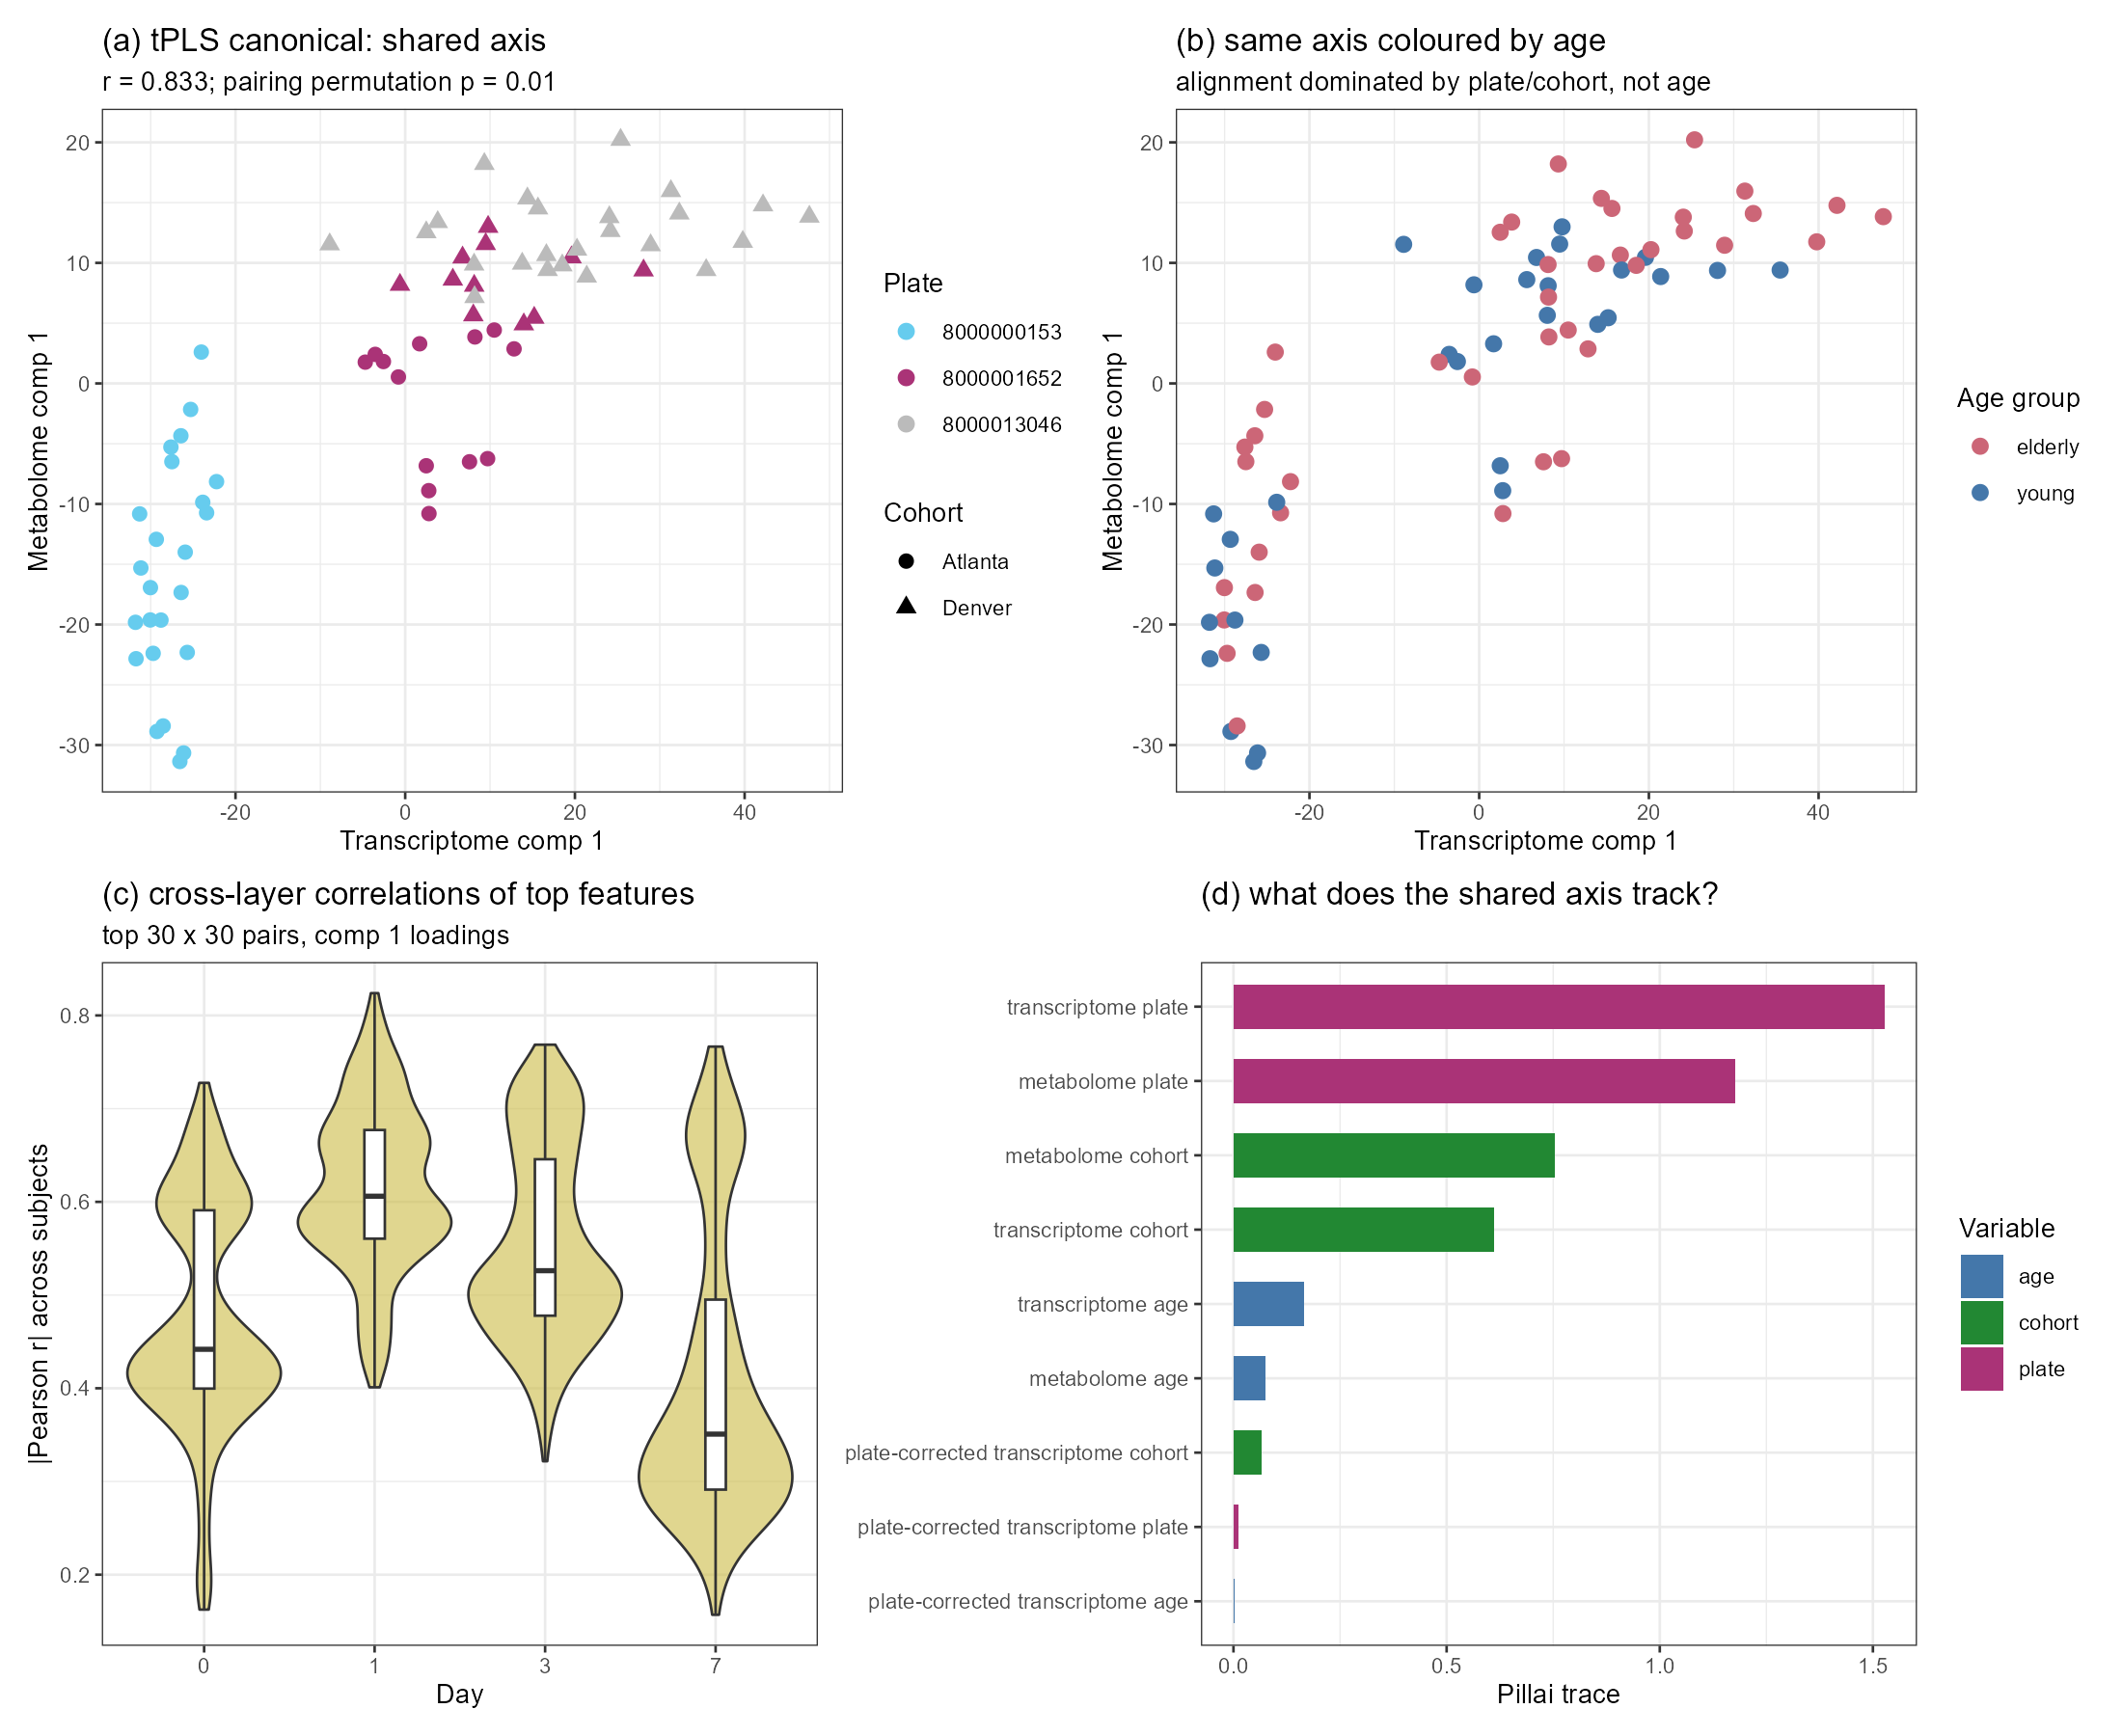
\includegraphics[keepaspectratio,alt={Multi-block integration. (a) tPLS canonical shared axis (r = 0.83), coloured by plate; (b) same axis coloured by age; (c) cross-layer correlation structure across days; (d) what the shared axis tracks (Pillai trace per label).}]{figures/FV4_multiblock.png}}
\caption{Multi-block integration. (a) tPLS canonical shared axis (r =
0.83), coloured by plate; (b) same axis coloured by age; (c) cross-layer
correlation structure across days; (d) what the shared axis tracks
(Pillai trace per label).}
\end{figure}

The multi-block machinery works: it finds the strongest coordinated
variation across molecular layers, and the audit layer identifies that
variation. On this dataset the coordinated axis is technical; the
demonstration is nonetheless the clearest multi-omic capability shown in
this report, and it extends the framework's published case studies to a
transcriptome--metabolome pair analysed with an explicit batch audit.

\section{7 Discussion}\label{discussion}

\subsection{7.1 Contributions of the tensor
view}\label{contributions-of-the-tensor-view}

\begin{enumerate}
\def\labelenumi{\arabic{enumi}.}
\tightlist
\item
  \textbf{The correct unit of analysis, with measurable consequences.}
  The subject-level representation is not cosmetic: with identical data
  and models, naive repeated-measures protocols inflated permutation
  significance by 13--47\(\times\) (fish
  0.008\$\to\(0.106; vaccine 0.002\)\to\$0.094) and cross-validated
  accuracy by 4--8 percentage points. In both datasets the
  subject-grouped tensor model gave the best grouped accuracy (vaccine
  0.685; fish 0.682 vs matrix-grouped 0.620 and leaking naive 0.660),
  while a simple ridge on flattened fish features remained the strongest
  continuous-outcome predictor (LOSO \(R^2\) = 0.380). The advantage is
  inferential correctness and accuracy measured on the correct unit, not
  universal predictive superiority.
\item
  \textbf{Detection workflows that matrix views hide.} tPCA exposed
  batch structure in two nested layers (cohort, then processing plate),
  reproducing and extending the methods paper's Appendix B workflow. The
  extension matters: a biological variable can be imbalanced at a finer
  batch level than the obvious label (here: age vs plate), and only the
  tensor decomposition made this visible at the level of individual
  subjects. Had the analysis stopped at cohort-level adjustment, the
  original (confounded) conclusion would have stood.
\item
  \textbf{Multi-omic integration over time.} tPLS canonical and
  block.tPLS-DA integrate layers while preserving trajectories,
  producing subject-level shared scores and interpretable loadings.
  Their output on this dataset is a strong shared axis (r = 0.83) that
  the audit layer assigns to technical structure --- a result that
  showcases both the machinery and the necessity of the audit.
\end{enumerate}

\subsection{7.2 Limits of the tensor
view}\label{limits-of-the-tensor-view}

\begin{itemize}
\tightlist
\item
  \textbf{Pseudo-replication is an inference problem.} The tensor
  representation removes the temptation, but the same protection is
  available to matrix analyses through subject-level permutation and
  grouped CV. What tensor methods provide is the natural \emph{default}:
  one point per subject.
\item
  \textbf{Batch confounding must be audited at the finest level.} Tensor
  decomposition made the plate structure visible, but its removal was a
  standard matrix operation (ComBat); and the confound was only
  detectable because plate information could be recovered from raw CEL
  names --- a reminder that preprocessing provenance is part of the
  analysis.
\item
  \textbf{Small n and annotation limits remain.} The vaccine dataset
  cannot adjudicate the age question (its age signal is inseparable from
  batch; its response associations are underpowered at
  \textbar r\textbar{} \textless{} 0.33). The fish dataset is two time
  points only --- the minimal tensor case --- and its gene-level
  conclusions are module-level at best.
\end{itemize}

\subsection{7.3 Biological
interpretation}\label{biological-interpretation}

\begin{itemize}
\tightlist
\item
  \textbf{Killifish.} Early-adult and 20-week fin transcriptome
  \emph{levels} carry a replicated association with lifespan (in-sample
  \(R^2\) \(\approx\) 0.5; bootstrap CI {[}0.43, 0.66{]}); the
  association is organised in coherent modules --- a circadian-clock
  axis with direction-consistent effects in 7/8 core clock genes, and a
  proteasome/ubiquitin axis --- rather than in the mitochondrial complex
  I theme of the original study, which is recovered only diffusely
  (1.60\(\times\) enrichment). The dataset does not support prediction
  or mechanism claims.
\item
  \textbf{Vaccine.} The transcriptomic age axis of GSE79396 is not
  separable from processing-plate batch at n = 72. Neither the
  inflammaging gene panel nor the BTM modules survive plate adjustment;
  the within-site heterogeneity pattern is consistent with the plate
  explanation. The originally reported systems-vaccinology biology
  {[}5{]} rests on a broader multi-assay design than this GEO matrix;
  nothing in the present reanalysis supports or refutes the study's
  integrated conclusions, but it does show that the transcriptomic age
  axis alone cannot carry them.
\end{itemize}

\subsection{7.4 A validation protocol for tensorOmics
applications}\label{a-validation-protocol-for-tensoromics-applications}

\textbf{Table 2. Recommended checks when applying tensorOmics.}

{\def\LTcaptype{none} % do not increment counter
\begin{longtable}[]{@{}
  >{\raggedright\arraybackslash}p{(\linewidth - 4\tabcolsep) * \real{0.3333}}
  >{\raggedright\arraybackslash}p{(\linewidth - 4\tabcolsep) * \real{0.3333}}
  >{\raggedright\arraybackslash}p{(\linewidth - 4\tabcolsep) * \real{0.3333}}@{}}
\toprule\noalign{}
\begin{minipage}[b]{\linewidth}\raggedright
\#
\end{minipage} & \begin{minipage}[b]{\linewidth}\raggedright
Check
\end{minipage} & \begin{minipage}[b]{\linewidth}\raggedright
Implementation used here
\end{minipage} \\
\midrule\noalign{}
\endhead
\bottomrule\noalign{}
\endlastfoot
1 & Reproduce any prior pipeline exactly & Correlations = 1.0000 on
component scores \\
2 & Permute at the subject level; report the naive scheme for contrast &
Refit under permuted labels; report both p-values \\
3 & For trajectory claims, permute time within subject & Fish time
reshuffle (p = 0.150) \\
4 & Cross-validate by leaving out subjects; never rows & Manual verified
projection; grouped LOSO \\
5 & Audit \emph{nested} batch structure; correct at the finest level;
replicate within batch & Cohort \(\to\) plate; ComBat; within-plate
test \\
6 & Report robustness grids, bootstrap CIs, multiplicity control and a
minimum detectable effect & Sensitivity; bootstrap; family-level FDR;
MDE = 0.325 \\
\end{longtable}
}

\subsection{7.5 Corrections relative to the first
report}\label{corrections-relative-to-the-first-report}

This report supersedes three statements of the earlier draft: (i) the
fish signal is level-based, not trajectory-based (Section 4.2); (ii) the
vaccine age axis and its inflammaging gene panel are confounded with
processing plate and are withdrawn as biological claims (Sections
5.2--5.3); (iii) response-level models are better described as
underpowered than as failures (Section 5.4). These corrections are the
direct product of the audit layer and illustrate its purpose.

\subsection{7.6 Limitations}\label{limitations}

Both datasets are analysed complete-case. The fish tensor is minimal
(two time points), so tensor-specific advantages over well-conducted
matrix analyses are modest there. The vaccine dataset is small (n = 72),
has one dominant technical confound, and only partial supplement
coverage for immune outcomes (Tfh n = 34). Metabolite features are
largely unidentified m/z--retention-time pairs, limiting biological
interpretation of the multi-block axis. The plate structure was
recovered from CEL file names rather than from curated metadata; while
the pattern is unambiguous, the analysis would have been cleaner with an
explicit batch field. The validation protocol itself (Section 3.4) is
designed for complete, matched designs; irregular sampling requires the
interpolation strategies discussed by the methods paper {[}1{]}.
Multiplicity was handled within each analysis's natural family using the
Benjamini-Hochberg procedure; applied to the stored statistics it leaves
every reported conclusion unchanged (individual gene-level calls inside
the exploratory joint reference families can shift at the threshold,
without affecting any reported conclusion). Families whose composition
follows a display table rather than a hypothesis --- the
scheme-comparison panel, the per-component summaries, the block-level
statistics of Section 6 --- remain exploratory and are treated as
descriptive. Fold-safe re-derivations were completed for the killifish
classification, baseline and regression models, for the pooled vaccine
LOSO, and for the within-cohort checks; deviations from the committed
values are documented in the repository's validation record, and the
fold-safe values are those cited in Sections 4 and 5.3.

\section{8 Conclusion}\label{conclusion}

Tensor-aware analysis is best read as a representation and workflow
layer rather than a replacement for matrix methods: it puts the subject
at the centre of the score plot, makes repeated-measures inference the
default, exposes nested technical structure, and enables multi-omic
integration over time. On the two datasets analysed here, that layer (a)
quantified two classical illusions --- pseudo-replication and batch
confounding --- that the earlier analysis had partly absorbed, (b)
supported a corrected and defensible biological conclusion in the
killifish data (a level-based, module-organised, replicated lifespan
association), and (c) converted a previously positive but confounded
vaccine result into a methodological case study. The most useful outcome
for future work is the validation protocol of Section 3.4: six checks
that are cheap to run, applicable to any tensorOmics application, and
able to separate exploratory structure from defensible evidence.

\section{Code and reporting note}\label{code-and-reporting-note}

All analyses were run locally with seeds fixed: the revision-stage
scripts live in \texttt{TER\_revision/scripts/} and the killifish
optimisation stage (``Task A'') in
\texttt{fish\_v2\_src/ter\_optimization/scripts/}; Appendix A maps each
results block to its producing scripts and stored result files. Most
numbers are stored as files under \texttt{results/tables/} or the
fish-stage results directory; a small number of diagnostic values exist
only as console output at the time of writing. Fish tensor analyses are
performed with the official R \texttt{tensorOmics} package plus a Python
audit pipeline (scikit-learn); vaccine analyses use the official R
package, mixOmics, sva and PLSDAbatch, with a verified manual projection
for held-out subject prediction. Code implementation, language
polishing, report organisation and code review were carried out with AI
assistance under the author's direction (the fish optimisation stage
used the ClawsGO Science Harness; the revision stage used a local coding
agent). All numerical values come from the executed scripts; most are
also stored as result files, and the few that exist only as console
output are flagged in the audit log. The analysis of the killifish
dataset builds on the earlier optimisation stage of the internship
(``Task A''), which has been re-executed and verified in this workspace
before inclusion.

\section{Appendix A. Traceability of reported
numbers}\label{appendix-a.-traceability-of-reported-numbers}

All numbers in this report were produced by the scripts in
\texttt{TER\_revision/scripts/} (fish optimisation stage:
\texttt{fish\_v2\_src/ter\_optimization/scripts/}); results blocks are
stored under \texttt{TER\_revision/results/tables/} and
\texttt{fish\_v2\_src/ter\_optimization/results/}, as mapped below. A
few diagnostic values exist only as console output and are not stored as
files.

{\def\LTcaptype{none} % do not increment counter
\begin{longtable}[]{@{}
  >{\raggedright\arraybackslash}p{(\linewidth - 4\tabcolsep) * \real{0.3333}}
  >{\raggedright\arraybackslash}p{(\linewidth - 4\tabcolsep) * \real{0.3333}}
  >{\raggedright\arraybackslash}p{(\linewidth - 4\tabcolsep) * \real{0.3333}}@{}}
\toprule\noalign{}
\begin{minipage}[b]{\linewidth}\raggedright
Report item
\end{minipage} & \begin{minipage}[b]{\linewidth}\raggedright
Main scripts
\end{minipage} & \begin{minipage}[b]{\linewidth}\raggedright
Result files
\end{minipage} \\
\midrule\noalign{}
\endhead
\bottomrule\noalign{}
\endlastfoot
Fish reproduction, permutation, LOSO, bootstrap, sensitivity, gene FDR &
\texttt{03\_fish\_analysis.py} & \texttt{TA\_summary.json},
\texttt{TA\_loso\_cv.csv}, \texttt{TA\_sensitivity.csv},
\texttt{TA\_gene\_fdr.csv.gz} \\
Fish annotation, complex I, circadian panel &
\texttt{01\_parse\_gff.py}, \texttt{04\_annotate\_hits.py} &
\texttt{gene\_annotation.tsv},
\texttt{TA\_top\_loadings\_annotated.csv},
\texttt{TA\_complexI\_members.csv}, \texttt{TA\_circadian\_genes.csv},
\texttt{TA\_enrichment\_summary.json} \\
Fish time-block ablation & \texttt{06\_ablation.py} &
\texttt{TA\_ablation.csv} \\
Fish GSEA (Enrichr) & \texttt{05\_fish\_figures\_gsea.py} &
\texttt{TA\_gsea\_enrichr.csv} \\
Fish matrix-vs-tensor comparison, permutation inflation, LOSO &
\texttt{07\_fish\_comparison.R}, \texttt{07b\_fish\_scores\_fix.R},
\texttt{07c\_fish\_tplsda\_loo.R} & \texttt{fish\_manova.csv},
\texttt{fish\_perm\_inflation.csv},
\texttt{fish\_loso\_naive\_vs\_grouped.csv},
\texttt{fish\_scores\_row.csv}, \texttt{fish\_scores\_subject.csv} \\
Fish tPLS regression (in-sample, permutation, LOSO) &
\texttt{08\_fish\_tpls\_regression.R} &
\texttt{fish\_tpls\_regression.csv} \\
Vaccine data preparation and v1 exact reproduction &
\texttt{10\_prepare\_gse79396.R}, \texttt{11\_reproduce\_v1.R} &
\texttt{repro\_v1\_check.txt}, \texttt{vaccine\_data.rds} \\
Vaccine value-proposition: MANOVA, permutation inflation, LOSO &
\texttt{20\_vaccine\_valueprop.R} & \texttt{vacc\_manova.csv},
\texttt{vacc\_perm\_inflation.csv}, \texttt{vacc\_loso.csv},
\texttt{vacc\_scores\_row.csv}, \texttt{vacc\_scores\_subject.csv} \\
Vaccine batch workflow (cohort, plate, within-site, 5-component checks)
& \texttt{21\_vaccine\_batch.R}, \texttt{21b–21d} &
\texttt{vacc\_batch\_metrics.csv}, \texttt{vacc\_within\_cohort.csv},
\texttt{vacc\_heterogeneity\_comps.csv},
\texttt{vacc\_chip\_correction.csv},
\texttt{vacc\_chip\_adjustment.csv}, \texttt{vacc\_chip\_tpca5.txt} \\
Vaccine gene panel, BTM modules, axis dynamics, response boundary &
\texttt{22\_vaccine\_deep.R}, \texttt{22b\_baseline\_dynamics.R} &
\texttt{vacc\_v1genes\_chip\_adjust.csv},
\texttt{vacc\_btm\_age\_chip.csv},
\texttt{vacc\_axis\_dynamics\_anova.csv}, \texttt{vacc\_boundary.csv},
\texttt{vacc\_mde.txt} \\
Multi-block integration (canonical, block.tPLS-DA, cross-layer, chip
sensitivity) & \texttt{30\_vaccine\_multiblock.R},
\texttt{30b\_multiblock\_corrected\_align.R} &
\texttt{vacc\_multiblock\_canonical.csv},
\texttt{vacc\_multiblock\_align.csv},
\texttt{vacc\_multiblock\_blocktplsda.csv},
\texttt{vacc\_multiblock\_crosslayer.csv},
\texttt{vacc\_multiblock\_scores.csv} \\
Figures & \texttt{40\_vaccine\_figures.R}, \texttt{41\_fish\_figures.R}
& \texttt{results/figures/FV1–FV4}, \texttt{FF1–FF2},
\texttt{FA1–FA5} \\
\end{longtable}
}

\section{References}\label{references}

{[}1{]} Kodikara S, Lu B, Wang S, Lê Cao K-A. tensorOmics: Data
integration for longitudinal omics data using tensor factorisation.
bioRxiv. 2026. doi:10.64898/2026.02.10.705179.

{[}2{]} Mor U, Cohen Y, Valdes-Mas R, Kviatcovsky D, Elinav E, Avron H.
Dimensionality reduction of longitudinal omics data using modern tensor
factorizations. PLOS Computational Biology. 2022;18(7):e1010212.
doi:10.1371/journal.pcbi.1010212.

{[}3{]} Rohart F, Gautier B, Singh A, Lê Cao K-A. mixOmics: An R package
for omics feature selection and multiple data integration. PLOS
Computational Biology. 2017;13(11):e1005752.
doi:10.1371/journal.pcbi.1005752.

{[}4{]} Baumgart M, Priebe S, Groth M, Hartmann N, Menzel U, Pandolfini
L, et al.~Longitudinal RNA-Seq analysis of vertebrate aging identifies
mitochondrial complex I as a small-molecule-sensitive modifier of
lifespan. Cell Systems. 2016;2(2):122--132.
doi:10.1016/j.cels.2016.01.014.

{[}5{]} Li S, Sullivan NL, Rouphael N, Yu T, Banton S, Maddur MS, et
al.~Metabolic phenotypes of response to vaccination in humans. Cell.
2017;169(5):862--877.e17. doi:10.1016/j.cell.2017.04.026.

{[}6{]} Johnson WE, Li C, Rabinovic A. Adjusting batch effects in
microarray expression data using empirical Bayes methods. Biostatistics.
2007;8(1):118--127. doi:10.1093/biostatistics/kxj037.

{[}7{]} Wang Y, Lê Cao K-A. PLSDA-batch: a multivariate framework to
correct for batch effects in microbiome data. Briefings in
Bioinformatics. 2023;24(2):bbac622. doi:10.1093/bib/bbac622.

\end{document}
